\documentclass[]{book}
\usepackage{lmodern}
\usepackage{amssymb,amsmath}
\usepackage{ifxetex,ifluatex}
\usepackage{fixltx2e} % provides \textsubscript
\ifnum 0\ifxetex 1\fi\ifluatex 1\fi=0 % if pdftex
  \usepackage[T1]{fontenc}
  \usepackage[utf8]{inputenc}
\else % if luatex or xelatex
  \ifxetex
    \usepackage{mathspec}
  \else
    \usepackage{fontspec}
  \fi
  \defaultfontfeatures{Ligatures=TeX,Scale=MatchLowercase}
\fi
% use upquote if available, for straight quotes in verbatim environments
\IfFileExists{upquote.sty}{\usepackage{upquote}}{}
% use microtype if available
\IfFileExists{microtype.sty}{%
\usepackage{microtype}
\UseMicrotypeSet[protrusion]{basicmath} % disable protrusion for tt fonts
}{}
\usepackage{hyperref}
\hypersetup{unicode=true,
            pdftitle={Predictive Modeling For Imposters},
            pdfauthor={Steve Pittard},
            pdfborder={0 0 0},
            breaklinks=true}
\urlstyle{same}  % don't use monospace font for urls
\usepackage{natbib}
\bibliographystyle{apalike}
\usepackage{color}
\usepackage{fancyvrb}
\newcommand{\VerbBar}{|}
\newcommand{\VERB}{\Verb[commandchars=\\\{\}]}
\DefineVerbatimEnvironment{Highlighting}{Verbatim}{commandchars=\\\{\}}
% Add ',fontsize=\small' for more characters per line
\usepackage{framed}
\definecolor{shadecolor}{RGB}{248,248,248}
\newenvironment{Shaded}{\begin{snugshade}}{\end{snugshade}}
\newcommand{\KeywordTok}[1]{\textcolor[rgb]{0.13,0.29,0.53}{\textbf{#1}}}
\newcommand{\DataTypeTok}[1]{\textcolor[rgb]{0.13,0.29,0.53}{#1}}
\newcommand{\DecValTok}[1]{\textcolor[rgb]{0.00,0.00,0.81}{#1}}
\newcommand{\BaseNTok}[1]{\textcolor[rgb]{0.00,0.00,0.81}{#1}}
\newcommand{\FloatTok}[1]{\textcolor[rgb]{0.00,0.00,0.81}{#1}}
\newcommand{\ConstantTok}[1]{\textcolor[rgb]{0.00,0.00,0.00}{#1}}
\newcommand{\CharTok}[1]{\textcolor[rgb]{0.31,0.60,0.02}{#1}}
\newcommand{\SpecialCharTok}[1]{\textcolor[rgb]{0.00,0.00,0.00}{#1}}
\newcommand{\StringTok}[1]{\textcolor[rgb]{0.31,0.60,0.02}{#1}}
\newcommand{\VerbatimStringTok}[1]{\textcolor[rgb]{0.31,0.60,0.02}{#1}}
\newcommand{\SpecialStringTok}[1]{\textcolor[rgb]{0.31,0.60,0.02}{#1}}
\newcommand{\ImportTok}[1]{#1}
\newcommand{\CommentTok}[1]{\textcolor[rgb]{0.56,0.35,0.01}{\textit{#1}}}
\newcommand{\DocumentationTok}[1]{\textcolor[rgb]{0.56,0.35,0.01}{\textbf{\textit{#1}}}}
\newcommand{\AnnotationTok}[1]{\textcolor[rgb]{0.56,0.35,0.01}{\textbf{\textit{#1}}}}
\newcommand{\CommentVarTok}[1]{\textcolor[rgb]{0.56,0.35,0.01}{\textbf{\textit{#1}}}}
\newcommand{\OtherTok}[1]{\textcolor[rgb]{0.56,0.35,0.01}{#1}}
\newcommand{\FunctionTok}[1]{\textcolor[rgb]{0.00,0.00,0.00}{#1}}
\newcommand{\VariableTok}[1]{\textcolor[rgb]{0.00,0.00,0.00}{#1}}
\newcommand{\ControlFlowTok}[1]{\textcolor[rgb]{0.13,0.29,0.53}{\textbf{#1}}}
\newcommand{\OperatorTok}[1]{\textcolor[rgb]{0.81,0.36,0.00}{\textbf{#1}}}
\newcommand{\BuiltInTok}[1]{#1}
\newcommand{\ExtensionTok}[1]{#1}
\newcommand{\PreprocessorTok}[1]{\textcolor[rgb]{0.56,0.35,0.01}{\textit{#1}}}
\newcommand{\AttributeTok}[1]{\textcolor[rgb]{0.77,0.63,0.00}{#1}}
\newcommand{\RegionMarkerTok}[1]{#1}
\newcommand{\InformationTok}[1]{\textcolor[rgb]{0.56,0.35,0.01}{\textbf{\textit{#1}}}}
\newcommand{\WarningTok}[1]{\textcolor[rgb]{0.56,0.35,0.01}{\textbf{\textit{#1}}}}
\newcommand{\AlertTok}[1]{\textcolor[rgb]{0.94,0.16,0.16}{#1}}
\newcommand{\ErrorTok}[1]{\textcolor[rgb]{0.64,0.00,0.00}{\textbf{#1}}}
\newcommand{\NormalTok}[1]{#1}
\usepackage{longtable,booktabs}
\usepackage{graphicx,grffile}
\makeatletter
\def\maxwidth{\ifdim\Gin@nat@width>\linewidth\linewidth\else\Gin@nat@width\fi}
\def\maxheight{\ifdim\Gin@nat@height>\textheight\textheight\else\Gin@nat@height\fi}
\makeatother
% Scale images if necessary, so that they will not overflow the page
% margins by default, and it is still possible to overwrite the defaults
% using explicit options in \includegraphics[width, height, ...]{}
\setkeys{Gin}{width=\maxwidth,height=\maxheight,keepaspectratio}
\IfFileExists{parskip.sty}{%
\usepackage{parskip}
}{% else
\setlength{\parindent}{0pt}
\setlength{\parskip}{6pt plus 2pt minus 1pt}
}
\setlength{\emergencystretch}{3em}  % prevent overfull lines
\providecommand{\tightlist}{%
  \setlength{\itemsep}{0pt}\setlength{\parskip}{0pt}}
\setcounter{secnumdepth}{5}
% Redefines (sub)paragraphs to behave more like sections
\ifx\paragraph\undefined\else
\let\oldparagraph\paragraph
\renewcommand{\paragraph}[1]{\oldparagraph{#1}\mbox{}}
\fi
\ifx\subparagraph\undefined\else
\let\oldsubparagraph\subparagraph
\renewcommand{\subparagraph}[1]{\oldsubparagraph{#1}\mbox{}}
\fi

%%% Use protect on footnotes to avoid problems with footnotes in titles
\let\rmarkdownfootnote\footnote%
\def\footnote{\protect\rmarkdownfootnote}

%%% Change title format to be more compact
\usepackage{titling}

% Create subtitle command for use in maketitle
\providecommand{\subtitle}[1]{
  \posttitle{
    \begin{center}\large#1\end{center}
    }
}

\setlength{\droptitle}{-2em}

  \title{Predictive Modeling For Imposters}
    \pretitle{\vspace{\droptitle}\centering\huge}
  \posttitle{\par}
    \author{Steve Pittard}
    \preauthor{\centering\large\emph}
  \postauthor{\par}
      \predate{\centering\large\emph}
  \postdate{\par}
    \date{2020-02-17}

\usepackage{booktabs}

\begin{document}
\maketitle

{
\setcounter{tocdepth}{1}
\tableofcontents
}
\chapter{Introduction}\label{intro}

This lecture is concerned primarily with Predictive Modeling. In this
domain there are generally two types of predictive models:

\begin{enumerate}
\def\labelenumi{\arabic{enumi})}
\tightlist
\item
  Classification for Predicting Qualitative Outcomes:
\end{enumerate}

This relates to situations such as whether someone has a disease
(``positive'') or not (``negative''). The problem could also be multi
classification such as assigning an organism to one of a number of
possible species.

\begin{enumerate}
\def\labelenumi{\arabic{enumi})}
\setcounter{enumi}{1}
\tightlist
\item
  Regression for Quantitative Out Comes
\end{enumerate}

This is when we wish to predict a numeric / continuous outcome such as a
final sales price for a house or car. It might also be a prediction of
tomorrow's stock or Bit Coin price.

\section{In-Sample vs Out-Of-Sample
Data}\label{in-sample-vs-out-of-sample-data}

The goal of predictive model is to generate models that can generalize
to new data. It would be good if any model we generate could provide a
good estimate of out of sample error. It's easy to generate a model on
an entire data set (in sample data) and then turn around and use that
data for prediction. But how will it perform on new data ? Haven't we
just over trained our model ?

\section{Performance Metrics}\label{performance-metrics}

For either case (regression vs classification) we need some type of
metric or measure to let us know how well a given model will work on new
or unseen data - also known as ``out of sample'' data. for
Classification problems we look at things like ``sensitivity'',
``specificity'', ``accuracy'', and ``Area Under Curve''. For
Quantitative outcomes, we look at things like Root Mean Square Error
(RMSE) or Mean Absolute Error (MAE). The selection of metric will
frequently depend on your domain of interest.

\chapter{Getting Hands On}\label{getting-hands-on}

Let's consider the Pima Indians Data that is part of the
\textbf{mlbench} package. You can install this package via the
\textbf{Tools -\textgreater{} Install Package} menu item within RStudio
or type the following at the R console prompt:

\begin{Shaded}
\begin{Highlighting}[]
\KeywordTok{install.packages}\NormalTok{(}\StringTok{"mlbench"}\NormalTok{)}
\end{Highlighting}
\end{Shaded}

Once you have it installed then load it into the work space as follows:

\begin{Shaded}
\begin{Highlighting}[]
\KeywordTok{data}\NormalTok{(}\StringTok{"PimaIndiansDiabetes"}\NormalTok{)}

\CommentTok{# Get a shorter handle. I hate typing. }
\NormalTok{pm <-}\StringTok{ }\NormalTok{PimaIndiansDiabetes}
\end{Highlighting}
\end{Shaded}

The description of the data set is as follows:

\begin{figure}
\centering
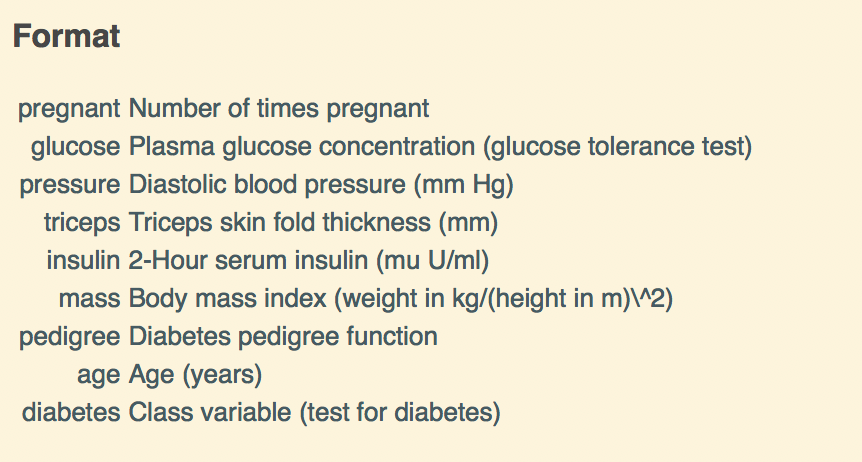
\includegraphics[width=4.94792in]{./PICS/pima_desc.png}
\caption{}
\end{figure}

So we now have some data on which we can build a model. Specifically,
there is a variable in the data called ``diabetes'' which indicates the
disease / diabetes status (``pos'' or ``neg'') of the person. It would
be good to come up with a model that we could use with incoming data to
determine if someone has diabetes.

\section{Important Terminology}\label{important-terminology}

In predictive modeling there are some common terms to consider:

\begin{figure}
\centering
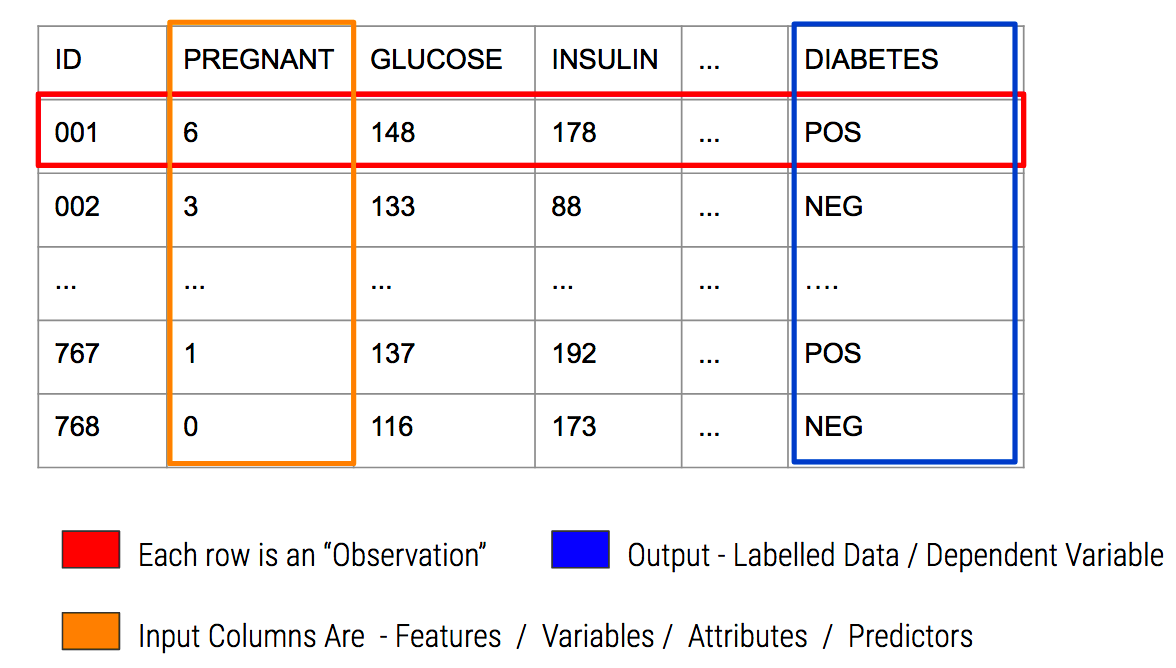
\includegraphics[width=4.94792in]{./PICS/features2.png}
\caption{}
\end{figure}

\section{Exploratory Plots}\label{exploratory-plots}

We'll look use some stock plots from the
\href{https://github.com/elastacloud/automatic-data-explorer}{\textbf{DataExplorer}}
package to get a feel for the data. Look at correlations between the
variables to see if any are strongly correlated with the variable we
wish to predict or any other variables.

\begin{Shaded}
\begin{Highlighting}[]
\KeywordTok{plot_correlation}\NormalTok{(pm, }\DataTypeTok{type=}\StringTok{"continuous"}\NormalTok{)}
\end{Highlighting}
\end{Shaded}

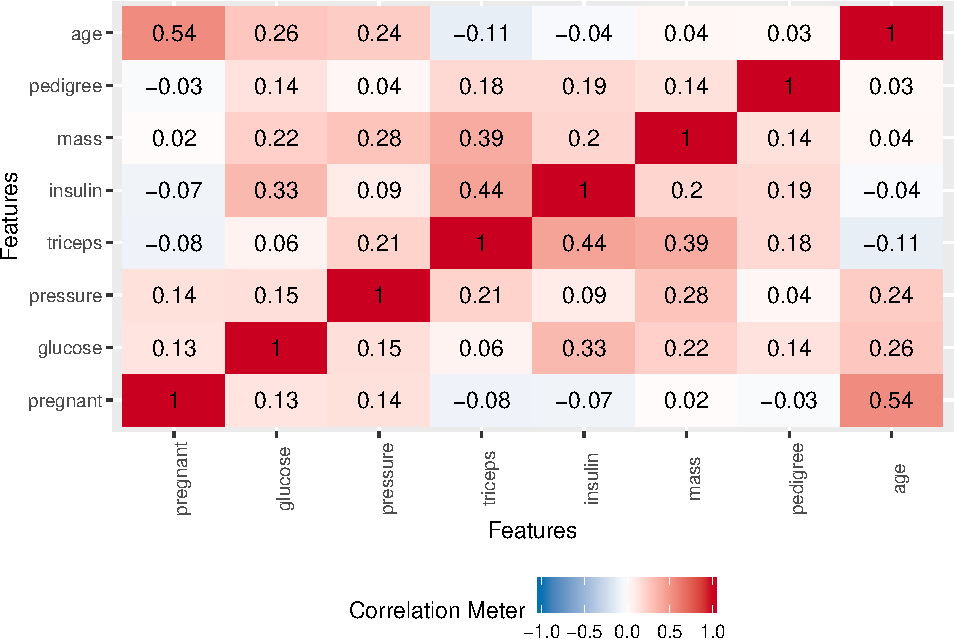
\includegraphics{SEMINAR_SERIES_files/figure-latex/decorr-1.pdf}

\begin{Shaded}
\begin{Highlighting}[]
\KeywordTok{plot_bar}\NormalTok{(pm)}
\end{Highlighting}
\end{Shaded}

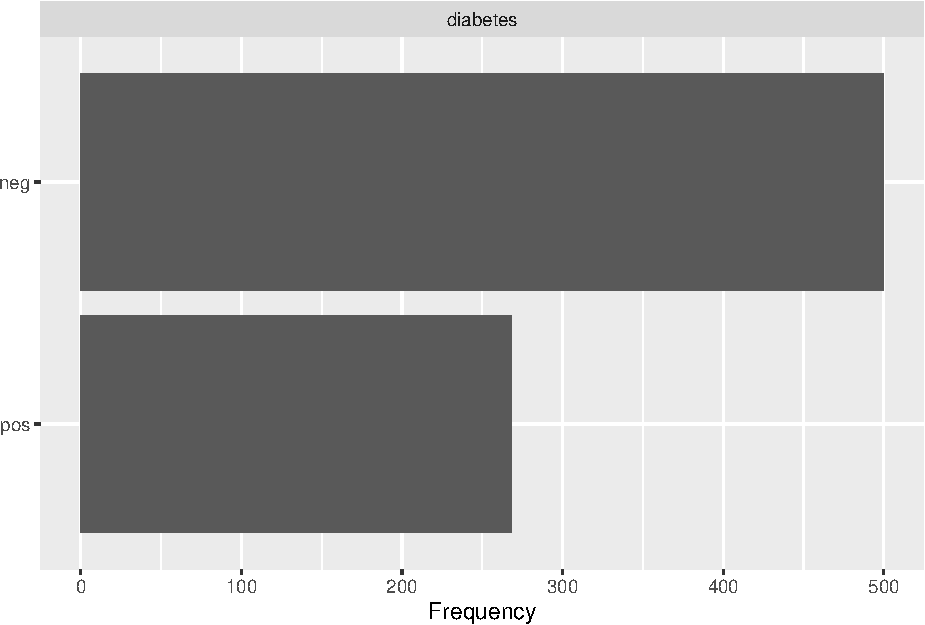
\includegraphics{SEMINAR_SERIES_files/figure-latex/debar-1.pdf}

\begin{Shaded}
\begin{Highlighting}[]
\KeywordTok{plot_histogram}\NormalTok{(pm)}
\end{Highlighting}
\end{Shaded}

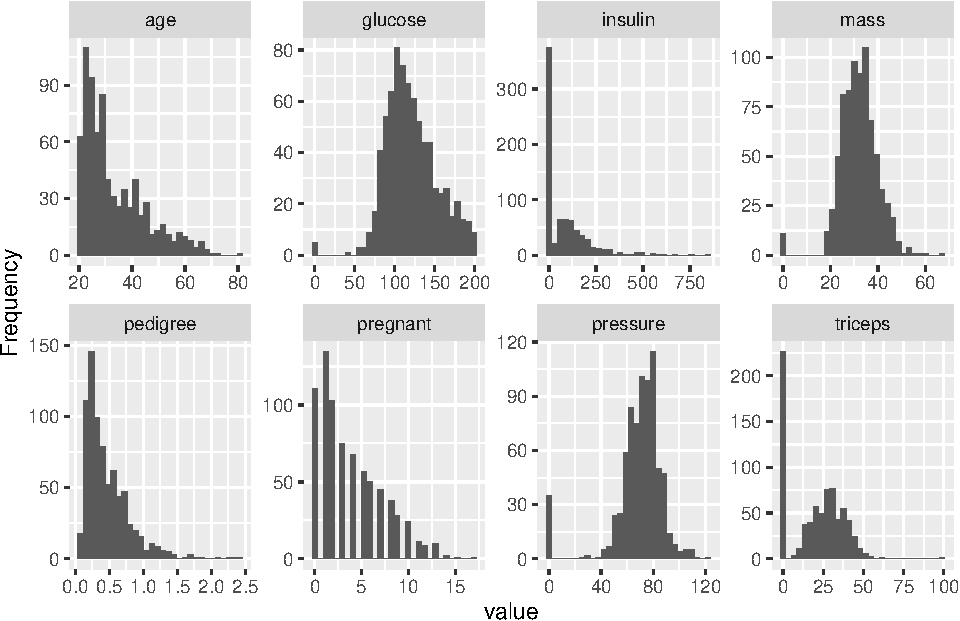
\includegraphics{SEMINAR_SERIES_files/figure-latex/phist-1.pdf}

\begin{Shaded}
\begin{Highlighting}[]
\KeywordTok{plot_boxplot}\NormalTok{(pm,}\DataTypeTok{by=}\StringTok{"diabetes"}\NormalTok{)}
\end{Highlighting}
\end{Shaded}

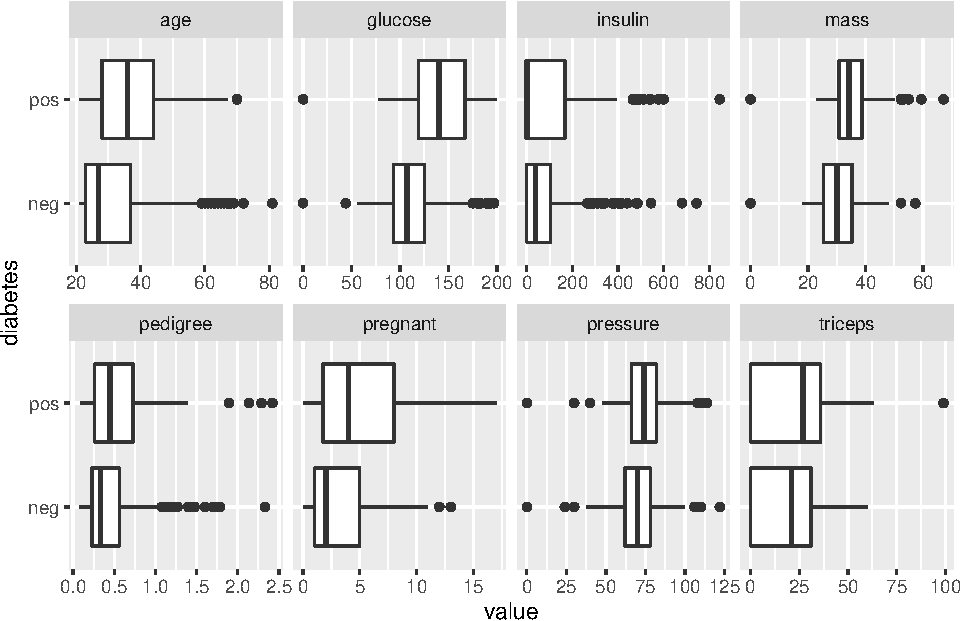
\includegraphics{SEMINAR_SERIES_files/figure-latex/pbox-1.pdf}

\chapter{A Common Modeling Workflow}\label{a-common-modeling-workflow}

The following graphic depicts the steps common to the Modeling Process.
This is not the only way to proceed but it provides a very helpful
schematic by which to plan your work.

\begin{figure}
\centering
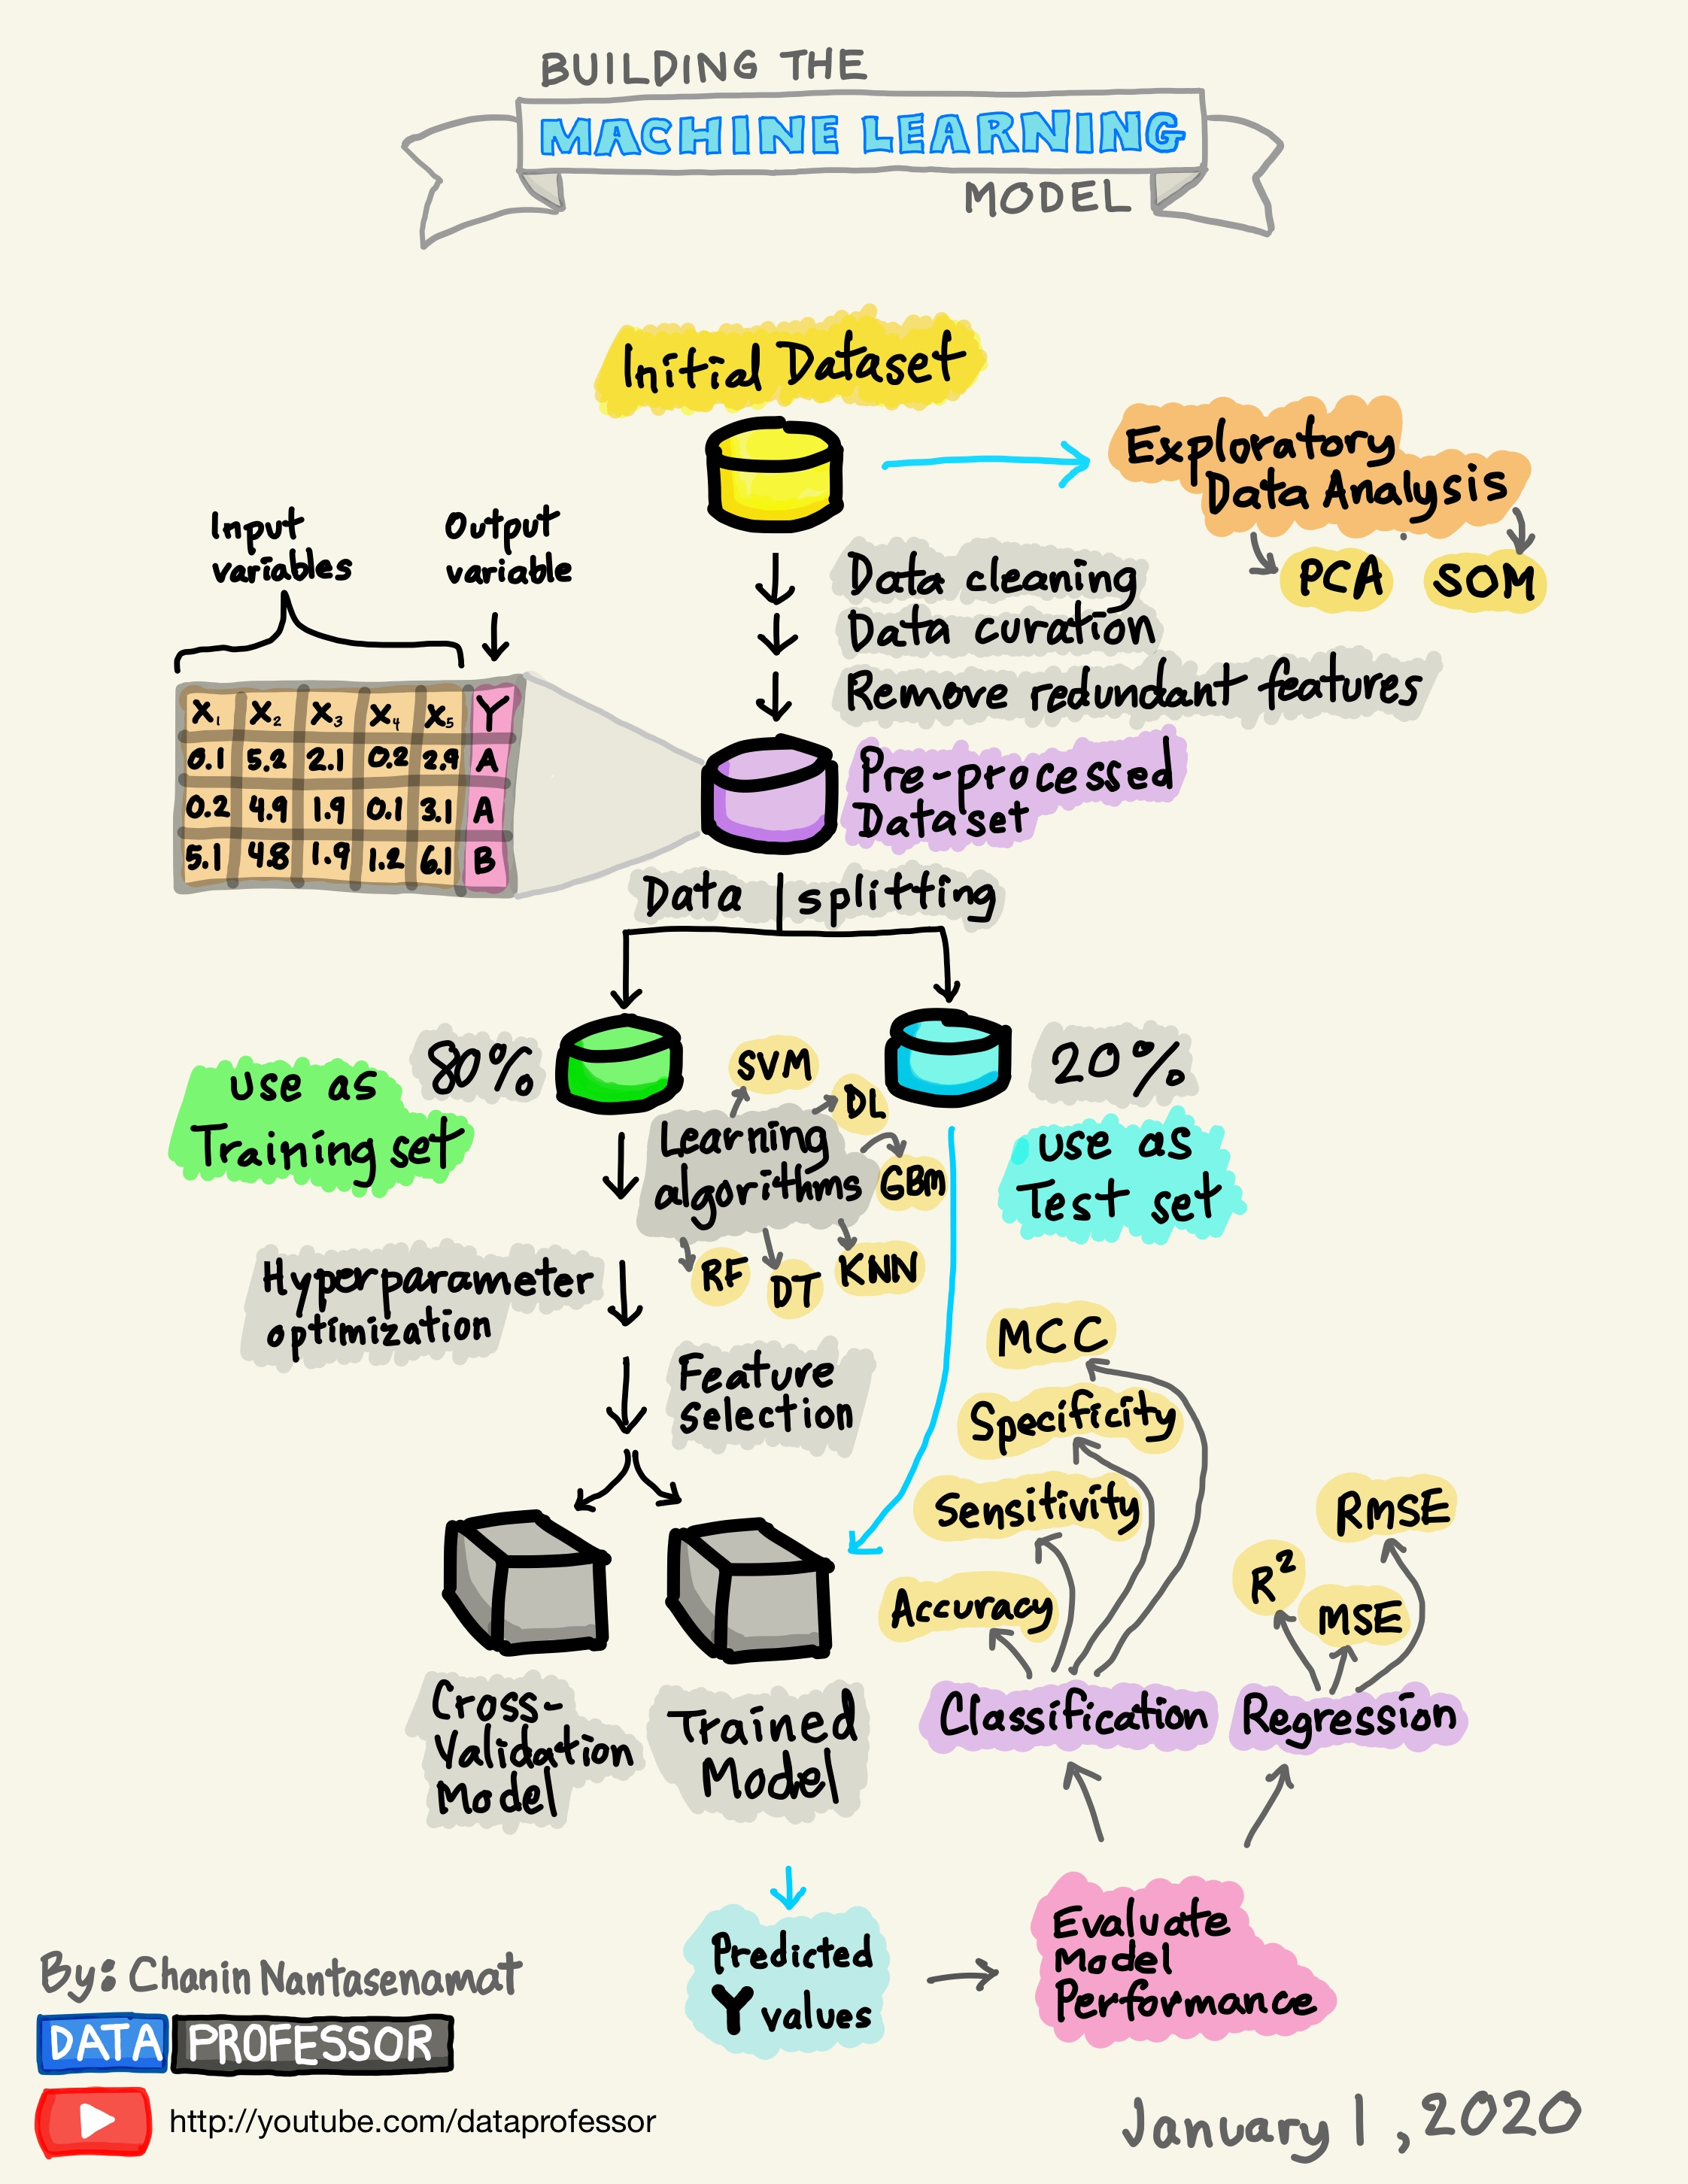
\includegraphics[height=6.25000in]{./PICS/sworkflow.jpg}
\caption{}
\end{figure}

\chapter{Splitting The Data}\label{splitting-the-data}

A fundamental approach used in ML is to segment data into a ``training''
set which is some percentage of the original data - say 80\%. The
remaining 20\% would be assigned to a ``test'' data set. Then we build a
model on our training data set after which we use that model to predict
outcomes for the test data set. This looks like the following.

\begin{figure}
\centering
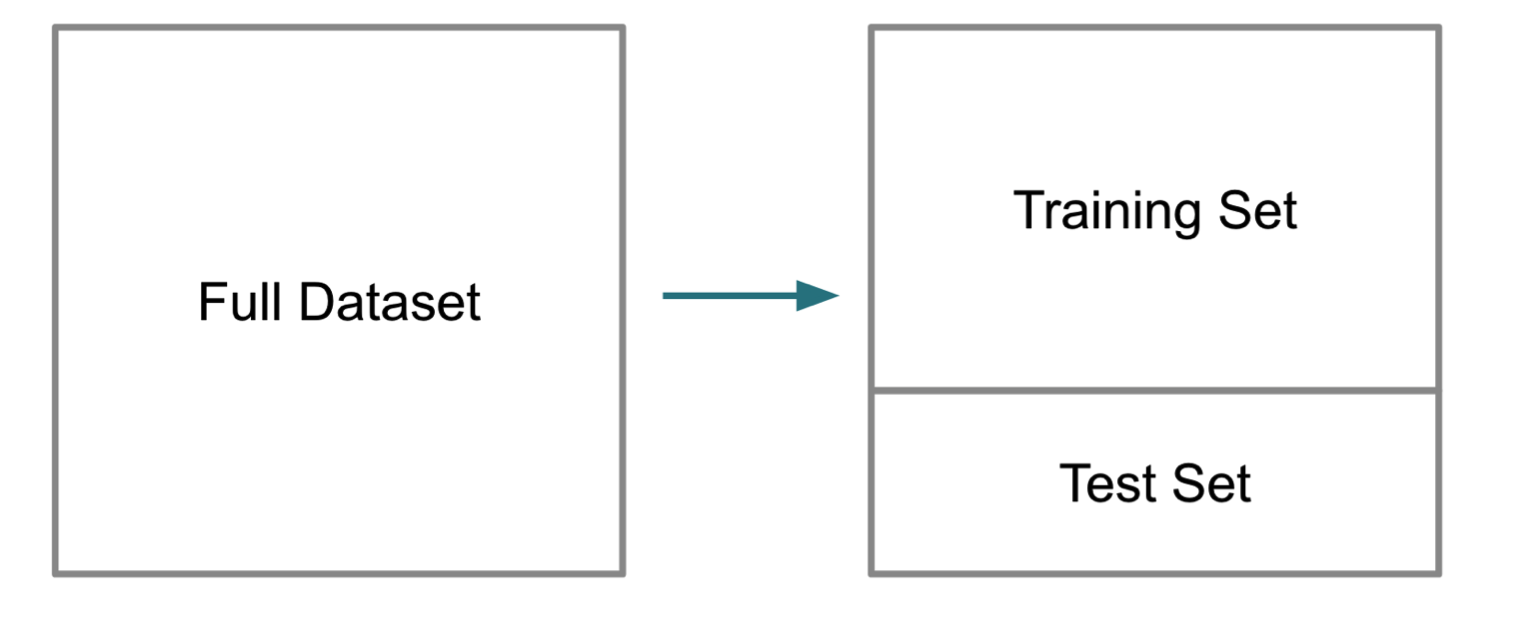
\includegraphics[width=5.20833in]{./PICS/crossvalid.png}
\caption{}
\end{figure}

Note that some scenarios will split the data into three data sets: 1)
training, 2) validation, and 3) test. This scenario is used when tuning
so called hyper parameters for methods that have ``tuning'' parameters
that could influence the resulting model. We'll stick with the basic
``train / test'' approach for now.

Splitting the data is not particularly challenging. We can use the built
in \textbf{sample} function in R to do this. We aren't sampling with
replacement here which guarantees that no record can exist in both sets.
That is, if a record from the data set is assigned to the training set,
it will not be in the test data set.

\begin{Shaded}
\begin{Highlighting}[]
\CommentTok{# Make this example reproducible}
\KeywordTok{set.seed}\NormalTok{(}\DecValTok{123}\NormalTok{) }
\NormalTok{percent <-}\StringTok{ }\NormalTok{.}\DecValTok{80}

\CommentTok{# Get the indices for a training set.}
\NormalTok{idx <-}\StringTok{ }\KeywordTok{sample}\NormalTok{(}\DecValTok{1}\OperatorTok{:}\KeywordTok{nrow}\NormalTok{(pm),}\KeywordTok{round}\NormalTok{(.}\DecValTok{8}\OperatorTok{*}\KeywordTok{nrow}\NormalTok{(pm)),F)}

\CommentTok{# Use bracket notation to create the train / test pair}
\NormalTok{train <-}\StringTok{ }\NormalTok{pm[idx,]}
\NormalTok{test  <-}\StringTok{ }\NormalTok{pm[}\OperatorTok{-}\NormalTok{idx,]}

\CommentTok{# The following should have 80 percent of the original }
\CommentTok{# data}

\KeywordTok{round}\NormalTok{(}\KeywordTok{nrow}\NormalTok{(train)}\OperatorTok{/}\KeywordTok{nrow}\NormalTok{(pm)}\OperatorTok{*}\DecValTok{100}\NormalTok{)}
\end{Highlighting}
\end{Shaded}

\begin{verbatim}
## [1] 80
\end{verbatim}

\section{First Model}\label{first-model}

Now let's build a Generalized Linear Model to do the prediction. We will
employ logistic regression.

\begin{Shaded}
\begin{Highlighting}[]
\NormalTok{myglm <-}\StringTok{ }\KeywordTok{glm}\NormalTok{(diabetes }\OperatorTok{~}\StringTok{ }\NormalTok{.,}
             \DataTypeTok{data =}\NormalTok{ train,}
             \DataTypeTok{family =} \StringTok{"binomial"}\NormalTok{)}

\KeywordTok{summary}\NormalTok{(myglm)}
\end{Highlighting}
\end{Shaded}

\begin{verbatim}
## 
## Call:
## glm(formula = diabetes ~ ., family = "binomial", data = train)
## 
## Deviance Residuals: 
##     Min       1Q   Median       3Q      Max  
## -2.3941  -0.7235  -0.4285   0.7476   3.0031  
## 
## Coefficients:
##               Estimate Std. Error z value Pr(>|z|)    
## (Intercept) -8.2308564  0.7816436 -10.530  < 2e-16 ***
## pregnant     0.1138202  0.0366475   3.106  0.00190 ** 
## glucose      0.0366854  0.0041947   8.746  < 2e-16 ***
## pressure    -0.0131360  0.0059415  -2.211  0.02704 *  
## triceps     -0.0006303  0.0075466  -0.084  0.93343    
## insulin     -0.0017394  0.0009826  -1.770  0.07667 .  
## mass         0.0847273  0.0161080   5.260 1.44e-07 ***
## pedigree     0.9057850  0.3329203   2.721  0.00651 ** 
## age          0.0120925  0.0107367   1.126  0.26005    
## ---
## Signif. codes:  0 '***' 0.001 '**' 0.01 '*' 0.05 '.' 0.1 ' ' 1
## 
## (Dispersion parameter for binomial family taken to be 1)
## 
##     Null deviance: 790.13  on 613  degrees of freedom
## Residual deviance: 581.40  on 605  degrees of freedom
## AIC: 599.4
## 
## Number of Fisher Scoring iterations: 5
\end{verbatim}

In looking at the output we see some problems such as a number of
predictors aren't significant so maybe we should eliminate them from the
model. For now, we'll keep going because we are trying to outline the
larger process / workflow.

\section{First Prediction}\label{first-prediction}

We could now use this new model to predict outcomes using the test data
set. Remember that we are attempting to predict a binary outcome - in
this case whether the person is positive for diabetes or negative.

What we get back from the prediction object are probabilities for which
we have to determine a threshold above which we would say the
observation is ``positive'' for diabetes and, below the threshold,
``negative''.

\begin{Shaded}
\begin{Highlighting}[]
\NormalTok{probs <-}\StringTok{ }\KeywordTok{predict}\NormalTok{(myglm,}
                 \DataTypeTok{newdata =}\NormalTok{ test,}
                 \DataTypeTok{type =} \StringTok{"response"}\NormalTok{)}

\NormalTok{probs[}\DecValTok{1}\OperatorTok{:}\DecValTok{10}\NormalTok{]}
\end{Highlighting}
\end{Shaded}

\begin{verbatim}
##         2         3         9        12        13        17        18 
## 0.0503311 0.8208652 0.6680994 0.9016430 0.7766679 0.3361188 0.2029466 
##        23        25        31 
## 0.9453408 0.6693923 0.4026717
\end{verbatim}

With logistic regression we are dealing with a curve like the one below
which is a sigmoid function. The idea is to take our probabilities,
which range between 0 and 1, and then pick a threshold over which we
would classify that person as being positive for diabetes.

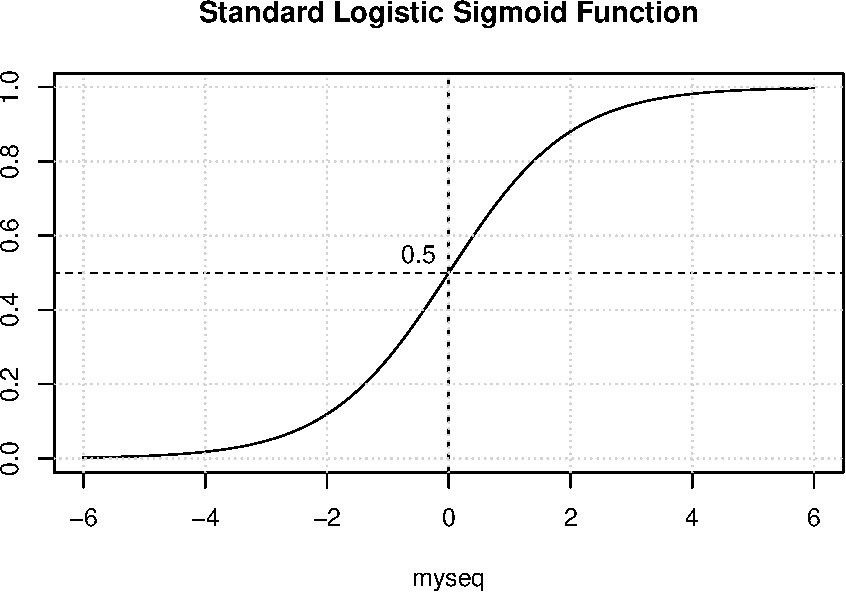
\includegraphics{SEMINAR_SERIES_files/figure-latex/logitplot-1.pdf}

\subsection{Selecting The Correct
Alpha}\label{selecting-the-correct-alpha}

The temptation is to select 0.5 as the threshold such that if a returned
probability exceeds 0.5 then we classify the associated subject as being
``positive'' for the disease. But then this assumes that the
probabilities are distributed accordingly. This is frequently not the
case though it doesn't stop people from using 0.5.

We might first wish to look at the distribution of the returned
probabilities before making a decision about where to set the threshold.
We can see clearly that selecting 0.5 in this case would not be
appropriate.

\begin{Shaded}
\begin{Highlighting}[]
\KeywordTok{boxplot}\NormalTok{(probs, }
        \DataTypeTok{main=}\StringTok{"Probabilities from our GLM Model"}\NormalTok{)}
\KeywordTok{grid}\NormalTok{()}
\end{Highlighting}
\end{Shaded}

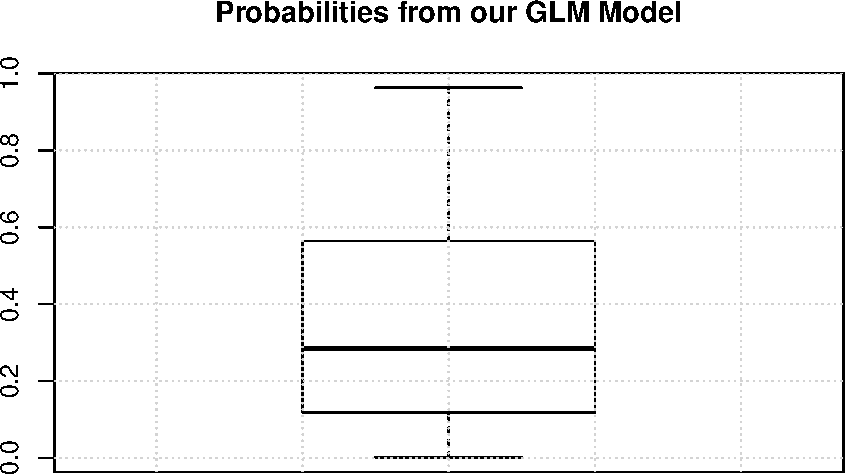
\includegraphics{SEMINAR_SERIES_files/figure-latex/bxplotalpha-1.pdf}

The median is somewhere around .25 so we could use that for now although
we are just guessing.

\begin{Shaded}
\begin{Highlighting}[]
\NormalTok{mypreds <-}\StringTok{ }\KeywordTok{ifelse}\NormalTok{(probs }\OperatorTok{>}\StringTok{ }\FloatTok{0.25}\NormalTok{,}\StringTok{"pos"}\NormalTok{,}\StringTok{"neg"}\NormalTok{)}
\NormalTok{mypreds <-}\StringTok{ }\KeywordTok{factor}\NormalTok{(mypreds, }\DataTypeTok{levels =} \KeywordTok{levels}\NormalTok{(test[[}\StringTok{"diabetes"}\NormalTok{]]))}
\NormalTok{mypreds[}\DecValTok{1}\OperatorTok{:}\DecValTok{10}\NormalTok{]}
\end{Highlighting}
\end{Shaded}

\begin{verbatim}
##   2   3   9  12  13  17  18  23  25  31 
## neg pos pos pos pos pos neg pos pos pos 
## Levels: neg pos
\end{verbatim}

\subsection{Confusion Matrices}\label{confusion-matrices}

Next, we would compare our predictions against the known outcomes which
are stored in the test data frame:

\begin{Shaded}
\begin{Highlighting}[]
\CommentTok{# How does this compare to the truth ?}
\KeywordTok{table}\NormalTok{(}\DataTypeTok{predicted =}\NormalTok{ mypreds,}
      \DataTypeTok{actual =}\NormalTok{ test}\OperatorTok{$}\NormalTok{diabetes)}
\end{Highlighting}
\end{Shaded}

\begin{verbatim}
##          actual
## predicted neg pos
##       neg  60   7
##       pos  37  50
\end{verbatim}

What we are doing is building a ``Confusion Matrix'' which can help us
determine how effective our model is. From such a matrix table we can
compute a number of ``performance measures'', such as accuracy,
precision, sensitivity, specificity and others, to help assess the
quality of the model. In predictive modeling we are always interested in
how well any given model will perform on ``new'' data.

There are some functions that can help us compute a confusion matrix.
Because the variable we are trying to predict, (diabetes), is a two
level factor, (``neg'' or ``pos'') we'll need to turn our predictions
into a comparable factor. Right now, it's just a character string.

\begin{Shaded}
\begin{Highlighting}[]
\CommentTok{# test$diabetes <- ordered(test$diabetes,c("pos","neg"))}

\NormalTok{mypreds <-}\StringTok{ }\KeywordTok{factor}\NormalTok{(mypreds,}
                  \DataTypeTok{levels=}\KeywordTok{levels}\NormalTok{(test}\OperatorTok{$}\NormalTok{diabetes))}

\NormalTok{caret}\OperatorTok{::}\KeywordTok{confusionMatrix}\NormalTok{(mypreds,test}\OperatorTok{$}\NormalTok{diabetes,}\DataTypeTok{positive=}\StringTok{"pos"}\NormalTok{)}
\end{Highlighting}
\end{Shaded}

\begin{verbatim}
## Confusion Matrix and Statistics
## 
##           Reference
## Prediction neg pos
##        neg  60   7
##        pos  37  50
##                                          
##                Accuracy : 0.7143         
##                  95% CI : (0.636, 0.7841)
##     No Information Rate : 0.6299         
##     P-Value [Acc > NIR] : 0.01718        
##                                          
##                   Kappa : 0.4472         
##                                          
##  Mcnemar's Test P-Value : 1.232e-05      
##                                          
##             Sensitivity : 0.8772         
##             Specificity : 0.6186         
##          Pos Pred Value : 0.5747         
##          Neg Pred Value : 0.8955         
##              Prevalence : 0.3701         
##          Detection Rate : 0.3247         
##    Detection Prevalence : 0.5649         
##       Balanced Accuracy : 0.7479         
##                                          
##        'Positive' Class : pos            
## 
\end{verbatim}

\section{Performance Measures
Revisited}\label{performance-measures-revisited}

This is helpful stuff although there are a number of measures to select
as a primary performance metric. Ideally, we would already know which
performance metric we would select to effectively ``judge'' the quality
of our model. In medical tests, ``sensitivity'' and ``specificity'' are
commonly used. Some applications use ``Accuracy'' (which isn't good when
there is large group imbalance). Anyway, if, for example, we pick
``sensitivity'' as a judge of model quality we see that is somewhere
around .87. (A much deeper discussion about selecting the best
performance measure is in order but we'll keep moving for now)

The problem here is that all we have done is looked at the confusion
matrix corresponding to one specific (and arbitrary) threshold value
when what we need is to look at a number of confusion matrices
corresponding to many different thresholds. For example, we might get a
better sensitivity level had we selected the mean of the returned
probabilities. This process could go on and on and on\ldots{} So we
would benefit from a rigorous approach to find the ``best'' threshold.

\section{The ROC curve}\label{the-roc-curve}

One way to do this is to use something known as the ROC curve. Luckily,
R has functions to do this. This isn't surprising as it is a standard
tool that has been in use for decades long before the hype of AI and ML
was around. The ROC curve gives us a ``one stop shop'' for estimating a
value of alpha that results in maximal area under a curve.

In fact, maximizing the area under a given ROC curve winds up being an
effective way to judge the differences between one method and another.
So, if we wanted to compare the glm model against a Support Vector
Machine model, we could use the respective AUC (Area Under Curve) metric
to help us. This isn't the only way to do this but it's reasonable for
now.

\begin{Shaded}
\begin{Highlighting}[]
\NormalTok{pred <-}\StringTok{ }\NormalTok{ROCR}\OperatorTok{::}\KeywordTok{prediction}\NormalTok{(}\DataTypeTok{predictions =}\NormalTok{ probs,}
                         \DataTypeTok{labels =}\NormalTok{ test}\OperatorTok{$}\NormalTok{diabetes)}

\NormalTok{perf <-}\StringTok{ }\KeywordTok{performance}\NormalTok{(pred,}
                    \StringTok{"tpr"}\NormalTok{,}
                    \StringTok{"fpr"}\NormalTok{)}
\KeywordTok{plot}\NormalTok{(perf,}\DataTypeTok{colorize=}\NormalTok{T,}
     \DataTypeTok{print.cutoffs.at=}\KeywordTok{seq}\NormalTok{(}\DecValTok{0}\NormalTok{,}\DecValTok{1}\NormalTok{,}\DataTypeTok{by=}\FloatTok{0.1}\NormalTok{),}
     \DataTypeTok{lwd=}\DecValTok{3}\NormalTok{,}\DataTypeTok{las=}\DecValTok{1}\NormalTok{,}\DataTypeTok{main=}\StringTok{"Cool ROC Curve"}\NormalTok{)}
\KeywordTok{abline}\NormalTok{(}\DataTypeTok{a =} \DecValTok{0}\NormalTok{, }\DataTypeTok{b =} \DecValTok{1}\NormalTok{)}

\KeywordTok{grid}\NormalTok{()}
\end{Highlighting}
\end{Shaded}

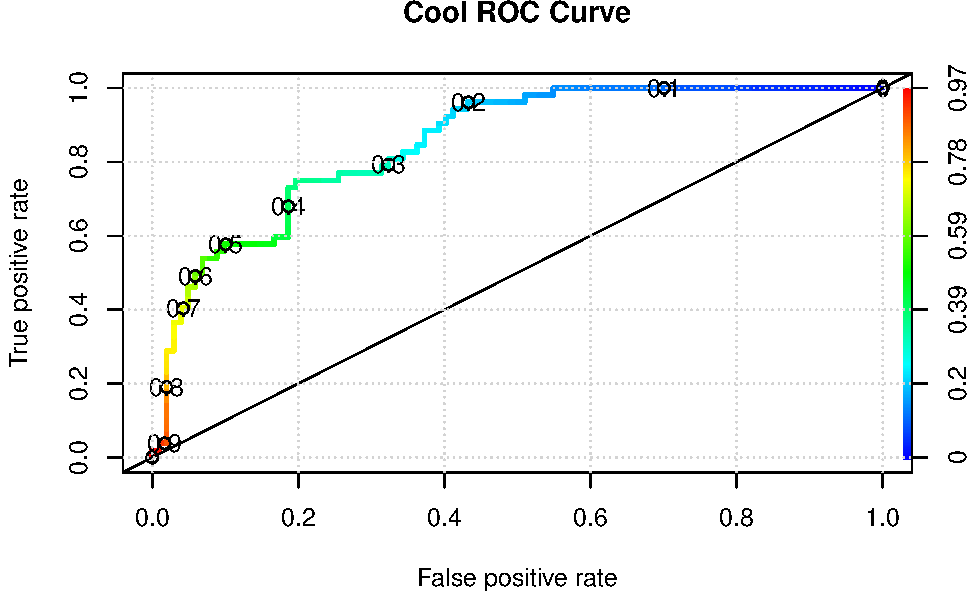
\includegraphics{SEMINAR_SERIES_files/figure-latex/rocrcalc-1.pdf}

\begin{Shaded}
\begin{Highlighting}[]
\NormalTok{myroc <-}\StringTok{ }\KeywordTok{performance}\NormalTok{(pred,}\DataTypeTok{measure=}\StringTok{"auc"}\NormalTok{)}
\NormalTok{myroc}\OperatorTok{@}\NormalTok{y.values[[}\DecValTok{1}\NormalTok{]]}
\end{Highlighting}
\end{Shaded}

\begin{verbatim}
## [1] 0.8507868
\end{verbatim}

So what value of alpha corresponds to the stated max AUC of .80 ? We'll
have to dig into the performance object to get that but it looks to be
between 0.30 and 0.40. Note that this is somewhat academic since knowing
the max AUC alone helps us decide if our model is any ``good''. For
completeness we could use another R function to nail this down:

\begin{Shaded}
\begin{Highlighting}[]
\KeywordTok{library}\NormalTok{(pROC)}
\NormalTok{proc <-}\StringTok{ }\KeywordTok{roc}\NormalTok{(test}\OperatorTok{$}\NormalTok{diabetes,probs)}
\KeywordTok{round}\NormalTok{(}\KeywordTok{coords}\NormalTok{(proc, }\StringTok{"b"}\NormalTok{, }\DataTypeTok{ret=}\StringTok{"t"}\NormalTok{, }\DataTypeTok{transpose =} \OtherTok{FALSE}\NormalTok{),}\DecValTok{2}\NormalTok{)}
\end{Highlighting}
\end{Shaded}

\begin{verbatim}
## [1] 0.35
\end{verbatim}

\chapter{Other Methods ?}\label{other-methods}

Well, we could use another method to see if it yields better performance
as determined by the AUC ? Let's use the \textbf{ranger} function which
is a fast implementation of random forests. One thing you will notice is
that we need to include the ``probability'' argument in the call to
ranger to get the necessary probabilities for computing the AUC. This is
one of the aggravations with using different functions. They all have
their own peculiar way of doing things.

\begin{Shaded}
\begin{Highlighting}[]
\KeywordTok{library}\NormalTok{(ranger)}
\NormalTok{ranger_mod <-}\StringTok{ }\KeywordTok{ranger}\NormalTok{(diabetes }\OperatorTok{~}\StringTok{ }\NormalTok{.,}
                   \DataTypeTok{data =}\NormalTok{ train,}
                   \DataTypeTok{probability =} \OtherTok{TRUE}\NormalTok{,}\DataTypeTok{mtry=}\DecValTok{4}\NormalTok{)}

\CommentTok{# Returns probabilities}
\NormalTok{ranger_pred <-}\StringTok{ }\KeywordTok{predict}\NormalTok{(ranger_mod,}\DataTypeTok{data=}\NormalTok{test)}

\NormalTok{myroc <-}\StringTok{ }\KeywordTok{roc}\NormalTok{(test}\OperatorTok{$}\NormalTok{diabetes,}
\NormalTok{             ranger_pred}\OperatorTok{$}\NormalTok{predictions[,}\DecValTok{2}\NormalTok{])}

\NormalTok{myroc}\OperatorTok{$}\NormalTok{auc}
\end{Highlighting}
\end{Shaded}

\begin{verbatim}
## Area under the curve: 0.8502
\end{verbatim}

\begin{Shaded}
\begin{Highlighting}[]
\NormalTok{pred <-}\StringTok{ }\NormalTok{ROCR}\OperatorTok{::}\KeywordTok{prediction}\NormalTok{(ranger_pred}\OperatorTok{$}\NormalTok{predictions[,}\DecValTok{2}\NormalTok{],}
\NormalTok{                         test}\OperatorTok{$}\NormalTok{diabetes)}
\NormalTok{perf <-}\StringTok{ }\KeywordTok{performance}\NormalTok{(pred,}
                    \StringTok{"tpr"}\NormalTok{,}
                    \StringTok{"fpr"}\NormalTok{)}
\KeywordTok{plot}\NormalTok{(perf,}\DataTypeTok{colorize=}\NormalTok{T,}
        \DataTypeTok{print.cutoffs.at=}\KeywordTok{seq}\NormalTok{(}\DecValTok{0}\NormalTok{,}\DecValTok{1}\NormalTok{,}\DataTypeTok{by=}\FloatTok{0.1}\NormalTok{),}
     \DataTypeTok{lwd=}\DecValTok{3}\NormalTok{,}\DataTypeTok{las=}\DecValTok{1}\NormalTok{,}\DataTypeTok{main=}\StringTok{"Cool ROC Curve"}\NormalTok{)}
\KeywordTok{abline}\NormalTok{(}\DataTypeTok{a =} \DecValTok{0}\NormalTok{, }\DataTypeTok{b =} \DecValTok{1}\NormalTok{)}

\KeywordTok{grid}\NormalTok{()}
\end{Highlighting}
\end{Shaded}

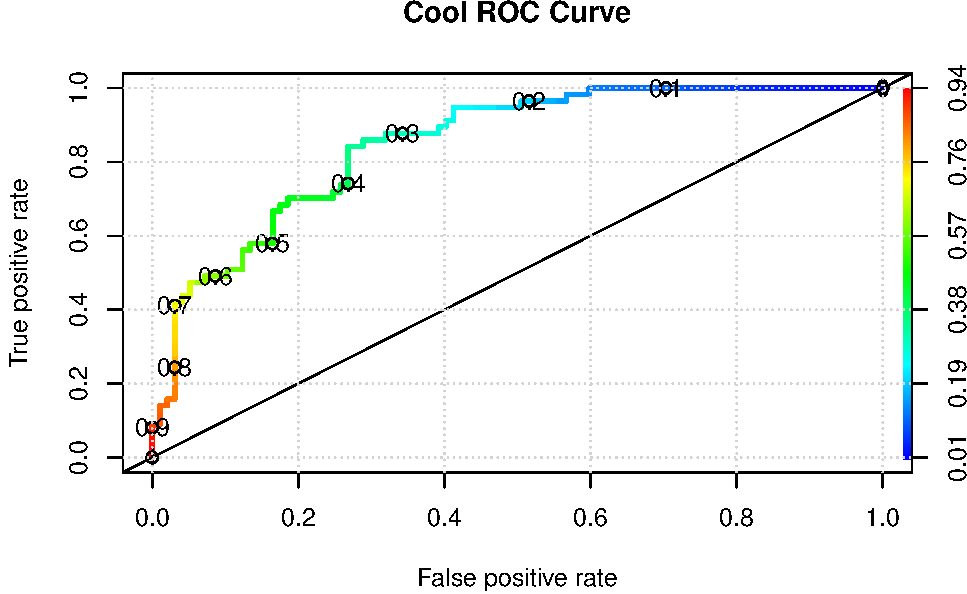
\includegraphics{SEMINAR_SERIES_files/figure-latex/range1-1.pdf}

\begin{Shaded}
\begin{Highlighting}[]
\NormalTok{rroc <-}\StringTok{ }\KeywordTok{performance}\NormalTok{(pred,}\DataTypeTok{measure=}\StringTok{"auc"}\NormalTok{)}
\NormalTok{rroc}\OperatorTok{@}\NormalTok{y.values[[}\DecValTok{1}\NormalTok{]]}
\end{Highlighting}
\end{Shaded}

\begin{verbatim}
## [1] 0.8502442
\end{verbatim}

It turns out that this didn't appear to improve things - at least with
one invocation of the method.

\section{Improving The Model(s)}\label{improving-the-models}

We haven't accomplished very much here because we need to look at
multiple versions of the data in case we sampled a number of outliers in
the creation of our training data. Or, maybe we have excluded a large
number of outliers in the training set so they wound up in the test data
set which means that the predictive power of our model isn't as robust
as it should be.

Our next steps should involve creating multiple versions of the training
and test pairs (say 3 times), compute the optimal AUC, and then look at
how those values vary for each of those individual versions. If the AUCs
vary widely then maybe our model is over training. If it's not varying
widely, it could be that that the model has high bias.

\section{Cross Fold Validation}\label{cross-fold-validation}

This is a method that gives us multiple estimates of out-of-sample
error, rather than a single estimate. In particular, we'll use an
approach called ``K-Fold Cross Validation'' where we will partition our
data into 3 individual ``folds''" which are basically equal in size.
Then we'll create a loop that does the following:

\begin{itemize}
\tightlist
\item
  Combines 2 of the folds into a training data set
\item
  Builds a model on the combined 2-folds data
\item
  Applies the model to holdout fold
\item
  Computes the AUC value and stores it
\end{itemize}

Each fold is simply a portion of the data. We'll generate a list called
``folds'' that contains 3 elements each of which are 256 index elements
corresponding to rows in pm. The way we did the sample insures that each
row shows up only in one fold.

\begin{figure}
\centering
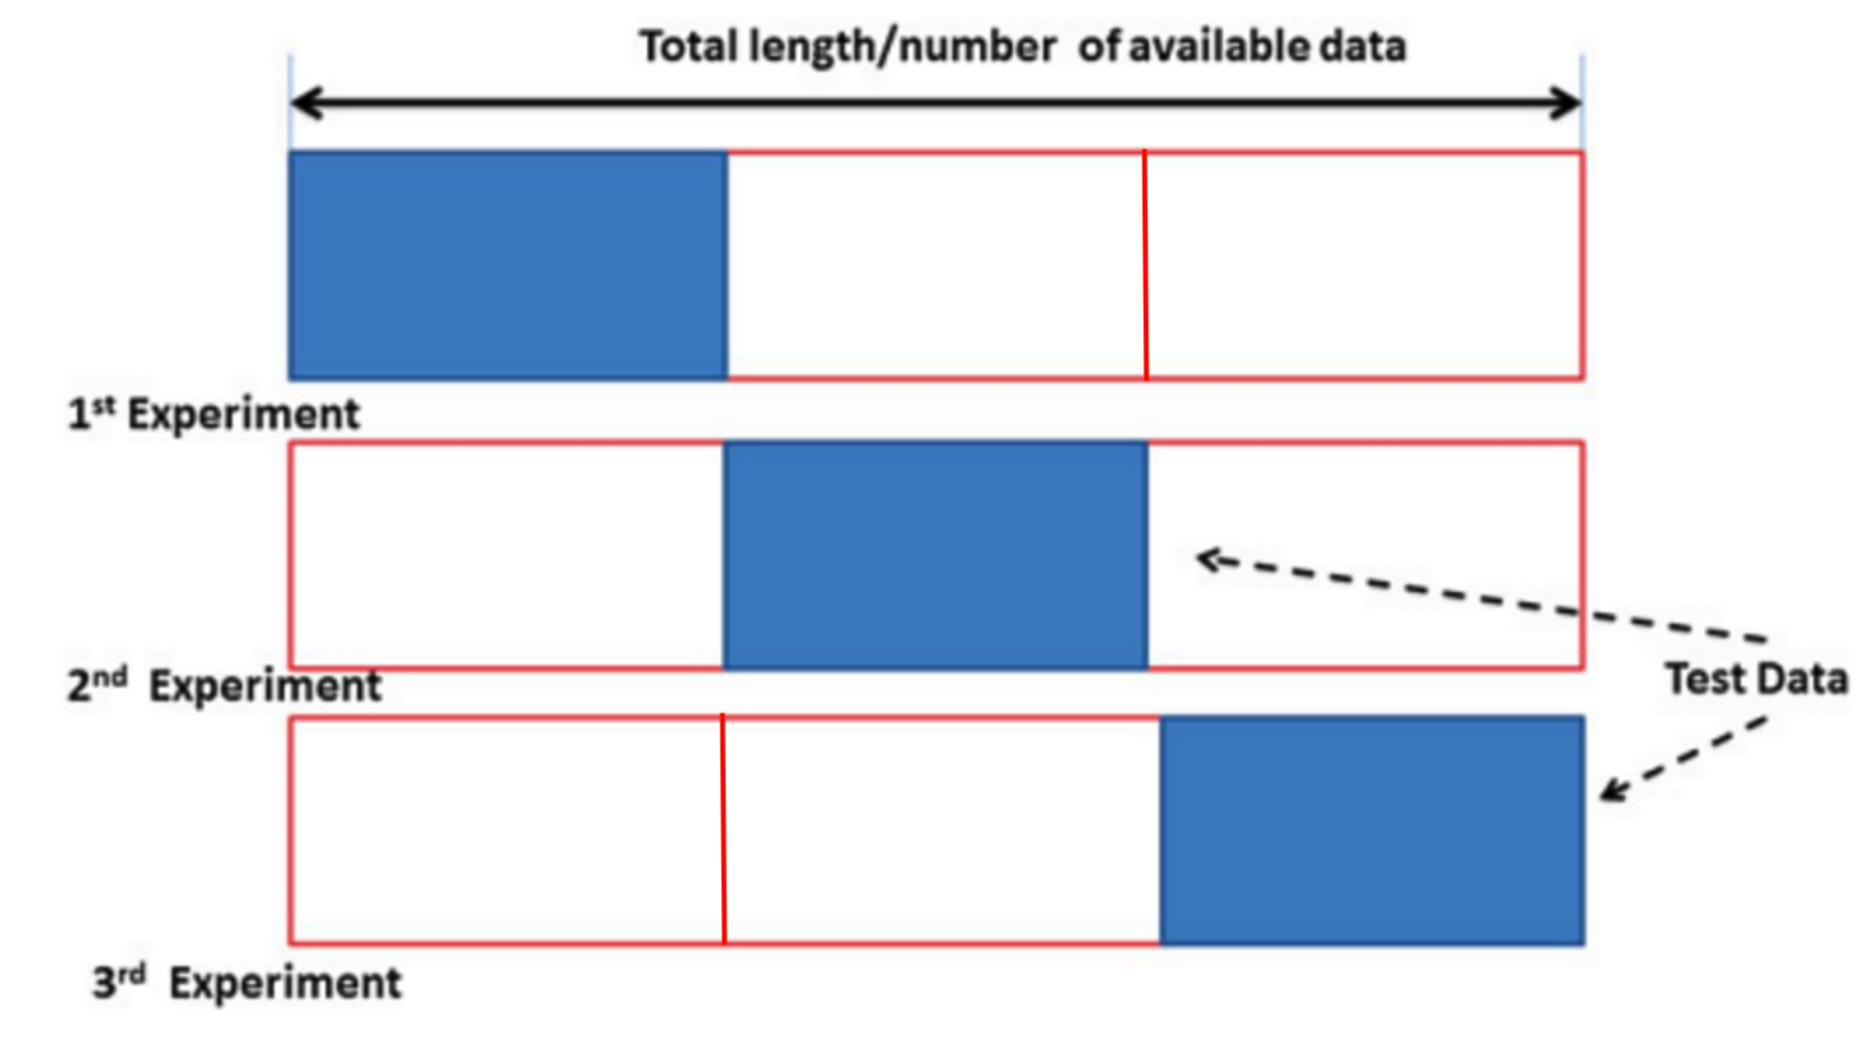
\includegraphics{./PICS/crossk.png}
\caption{}
\end{figure}

To drive this home, and in case the graphic didn't help, consider the
following simple data frame:

\begin{verbatim}
##   id   m1   m2   m3
## 1 a1 0.89 0.36 0.10
## 2 b2 0.75 0.27 0.22
## 3 c3 0.98 0.85 0.95
## 4 d4 0.04 0.36 0.75
## 5 e5 0.90 0.30 0.82
## 6 f6 0.87 0.76 0.42
## 7 g7 0.78 0.84 0.59
## 8 h8 0.38 0.46 0.80
## 9 i9 0.04 0.73 0.89
\end{verbatim}

If we created three folds out of this data frame it would look like the
following:

\begin{figure}
\centering
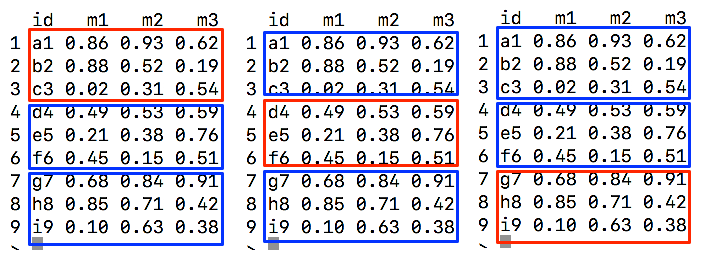
\includegraphics{./PICS/crossfold.png}
\caption{}
\end{figure}

Here is our function to implement the K-Fold validation. It's pretty
straightforward to define in terms of coding though it winds up being
somewhat specific to the particular method we are using.

\begin{Shaded}
\begin{Highlighting}[]
\NormalTok{cross_fold <-}\StringTok{ }\ControlFlowTok{function}\NormalTok{(}\DataTypeTok{numofolds =} \DecValTok{3}\NormalTok{) \{}
  
  \CommentTok{# Function to Do Cross fold validation}
  
  \CommentTok{# Split the data into K folds (numofolds)}
  
\NormalTok{  folds <-}\StringTok{ }\KeywordTok{split}\NormalTok{(}\KeywordTok{sample}\NormalTok{(}\DecValTok{1}\OperatorTok{:}\KeywordTok{nrow}\NormalTok{(pm)),}\DecValTok{1}\OperatorTok{:}\NormalTok{numofolds) }
  
  \CommentTok{# We setup some blank lists to stash results}
\NormalTok{  folddf    <-}\StringTok{ }\KeywordTok{list}\NormalTok{()  }\CommentTok{# Contains folds}
\NormalTok{  modl      <-}\StringTok{ }\KeywordTok{list}\NormalTok{()  }\CommentTok{# Hold each of the K models}
\NormalTok{  predl     <-}\StringTok{ }\KeywordTok{list}\NormalTok{()  }\CommentTok{# Hold rach of the K predictions}
\NormalTok{  auc       <-}\StringTok{ }\KeywordTok{list}\NormalTok{()  }\CommentTok{# Hold the auc for a given model}
  
  \CommentTok{# Create a formula that can be used across multiple}
  \CommentTok{# iterations through the loop. }
  
\NormalTok{  myform <-}\StringTok{ "diabetes ~ ."}
  
  \ControlFlowTok{for}\NormalTok{ (ii }\ControlFlowTok{in} \DecValTok{1}\OperatorTok{:}\KeywordTok{length}\NormalTok{(folds)) \{}
    
    \CommentTok{# This list holds the actual model we create for each of the }
    \CommentTok{# 10 folds}
    
\NormalTok{    modl[[ii]] <-}\StringTok{ }\KeywordTok{glm}\NormalTok{(}\DataTypeTok{formula =}\NormalTok{ myform, }
                      \DataTypeTok{data =}\NormalTok{ pm[}\OperatorTok{-}\NormalTok{folds[[ii]],],}
                      \DataTypeTok{family =} \StringTok{"binomial"}
\NormalTok{    )}
    
    \CommentTok{# This list will contain / hold the models build on the fold}
    
\NormalTok{    predl[[ii]]  <-}\StringTok{ }\KeywordTok{predict}\NormalTok{(modl[[ii]],}
                            \DataTypeTok{newdata=}\NormalTok{pm[folds[[ii]],],}
                            \DataTypeTok{type=}\StringTok{"response"}\NormalTok{)}
    
    \CommentTok{# This list will hold the results of the AUC per iteration}
    
\NormalTok{    pred <-}\StringTok{ }\NormalTok{ROCR}\OperatorTok{::}\KeywordTok{prediction}\NormalTok{(predl[[ii]],}
\NormalTok{                             pm[folds[[ii]],]}\OperatorTok{$}\NormalTok{diabetes)}
    
\NormalTok{    roc  <-}\StringTok{ }\KeywordTok{performance}\NormalTok{(pred,}\DataTypeTok{measure=}\StringTok{"auc"}\NormalTok{)}
\NormalTok{    auc[[ii]] <-}\StringTok{ }\NormalTok{roc}\OperatorTok{@}\NormalTok{y.values[[}\DecValTok{1}\NormalTok{]]}
\NormalTok{  \}}
  \KeywordTok{return}\NormalTok{(}\KeywordTok{unlist}\NormalTok{(auc))}
\NormalTok{\}}
\end{Highlighting}
\end{Shaded}

Running this is now quite simple. By default, this function will loop
three times corresponding to the number of folds. During each iteration
it will:

\begin{itemize}
\tightlist
\item
  use glm to build a model on the training folds
\item
  create a prediction object using the training fold
\item
  compute the underlying AUC associated with the prediction
\item
  store the AUC in a vector
\end{itemize}

At the end of the function, the vector containing the computed AUCs will
be returned.

\begin{Shaded}
\begin{Highlighting}[]
\KeywordTok{cross_fold}\NormalTok{()}
\end{Highlighting}
\end{Shaded}

\begin{verbatim}
## [1] 0.8628023 0.8050426 0.8115884
\end{verbatim}

\begin{Shaded}
\begin{Highlighting}[]
\CommentTok{# Use more folds}

\KeywordTok{cross_fold}\NormalTok{(}\DecValTok{8}\NormalTok{)}
\end{Highlighting}
\end{Shaded}

\begin{verbatim}
## [1] 0.7619048 0.8842505 0.8476583 0.8727273 0.8866224 0.7475586 0.8633959
## [8] 0.7528463
\end{verbatim}

We could take the average of the AUCs to get a sense of how well this
method would apply to unseen data.

\begin{Shaded}
\begin{Highlighting}[]
\KeywordTok{stripplot}\NormalTok{(}\KeywordTok{cross_fold}\NormalTok{(}\DecValTok{8}\NormalTok{),}
          \DataTypeTok{main=}\StringTok{"AUC values for K-Fold Validation"}\NormalTok{,}
          \DataTypeTok{type=}\KeywordTok{c}\NormalTok{(}\StringTok{"g"}\NormalTok{,}\StringTok{"p"}\NormalTok{),}\DataTypeTok{pch=}\DecValTok{19}\NormalTok{,}\DataTypeTok{cex=}\FloatTok{1.5}\NormalTok{)}
\end{Highlighting}
\end{Shaded}

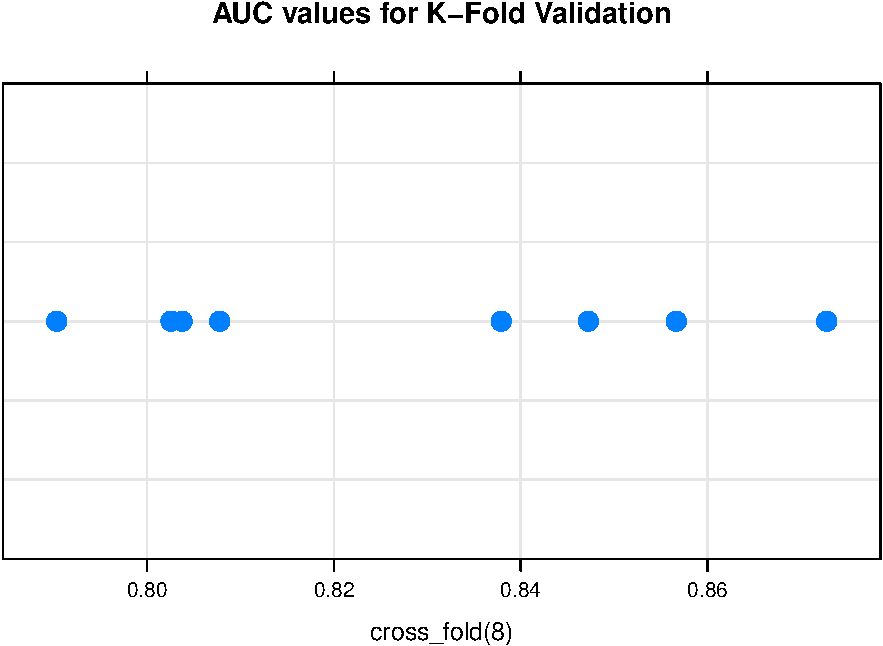
\includegraphics{SEMINAR_SERIES_files/figure-latex/strip1-1.pdf}

\chapter{Is There a Better Way ?}\label{is-there-a-better-way}

In R, as well as with Python, there are a growing number of packages
available to help simplify repetitive processes. Building predictive
models is no exception especially given that so many sub processes are
involved such as splitting data, building a model, making a prediction,
comparing it to the labelled data, and so on. The \textbf{caret} package
provides an easy point of entry into the world of predictive modeling.
It provides the following features:

\begin{verbatim}
- Streamlined and consistent syntax for more than 
  200 different models
- Can implement any of the 238 different methods using a single function
- Easy data splitting to simplify the creation of train / test pairs
- Realistic model estimates through built-in resampling
- Convenient feature importance determination
- Easy selection of different performance metrics (e.g. "ROC","Accuracy", "Sensitivity")
- Automated and semi-automated parameter tuning
- Simplifed comparison of different models
\end{verbatim}

The caret package was designed specifically for predictive modeling and,
in particular, to provide an intuitive approach to creating, managing,
and comparing different models emerging from various methods. Let's work
through our previous examples using functions from \textbf{caret}.

\section{Data Splitting Using Caret}\label{data-splitting-using-caret}

Let's split the data into a training / test pair. The caret package
provides some useful functions for this one of which is the
\textbf{CreateDataPartion} function.

\begin{Shaded}
\begin{Highlighting}[]
\NormalTok{idx <-}\StringTok{ }\KeywordTok{createDataPartition}\NormalTok{(pm}\OperatorTok{$}\NormalTok{diabetes,}
                           \DataTypeTok{p=}\NormalTok{.}\DecValTok{80}\NormalTok{,}
                           \DataTypeTok{list=}\OtherTok{FALSE}\NormalTok{)}

\NormalTok{Train <-}\StringTok{ }\NormalTok{pm[idx,]}
\NormalTok{Test  <-}\StringTok{ }\NormalTok{pm[}\OperatorTok{-}\NormalTok{idx,]}

\KeywordTok{nrow}\NormalTok{(Train)}
\end{Highlighting}
\end{Shaded}

\begin{verbatim}
## [1] 615
\end{verbatim}

Now we can use this to create a training object with caret. We'll create
a GLM model similar to the one we've already created. The primary, and
most frequently used, function in \textbf{caret} is the \textbf{train}
function. In this example we'll use it build a model using the
\textbf{glm} method. We will also specify that ``Accuracy'' will be the
preferred performance measure.

\begin{Shaded}
\begin{Highlighting}[]
\NormalTok{myglm_caret <-}\StringTok{ }\KeywordTok{train}\NormalTok{(diabetes }\OperatorTok{~}\StringTok{ }\NormalTok{.,}
                     \DataTypeTok{data =}\NormalTok{ Train,}
                     \DataTypeTok{method =} \StringTok{"glm"}\NormalTok{,}
                     \DataTypeTok{metric =} \StringTok{"Accuracy"}\NormalTok{)}
\NormalTok{myglm_caret}
\end{Highlighting}
\end{Shaded}

\begin{verbatim}
## Generalized Linear Model 
## 
## 615 samples
##   8 predictor
##   2 classes: 'neg', 'pos' 
## 
## No pre-processing
## Resampling: Bootstrapped (25 reps) 
## Summary of sample sizes: 615, 615, 615, 615, 615, 615, ... 
## Resampling results:
## 
##   Accuracy   Kappa    
##   0.7690868  0.4716828
\end{verbatim}

\section{Specifying Control Options}\label{specifying-control-options}

We can even request cross fold validation without having to write our
own function to do this. To do this requires the specification of a
``control'' object which contains information that we would like for the
\textbf{train} function to consider as it does its work.

Not every invocation of \textbf{train} requires an associated
\textbf{trainControl} object although as you become more experienced
building models, you will frequently use this approach.

\begin{Shaded}
\begin{Highlighting}[]
\NormalTok{control <-}\StringTok{ }\KeywordTok{trainControl}\NormalTok{(}\DataTypeTok{method =} \StringTok{"cv"}\NormalTok{, }\DataTypeTok{number =} \DecValTok{5}\NormalTok{)}

\NormalTok{myglm_caret <-}\StringTok{ }\KeywordTok{train}\NormalTok{(diabetes }\OperatorTok{~}\StringTok{ }\NormalTok{.,}
                     \DataTypeTok{data =}\NormalTok{ Train,}
                     \DataTypeTok{method =} \StringTok{"glm"}\NormalTok{,}
                     \DataTypeTok{metric =} \StringTok{"Accuracy"}\NormalTok{,}
                     \DataTypeTok{trControl =}\NormalTok{ control)}
\NormalTok{myglm_caret}
\end{Highlighting}
\end{Shaded}

\begin{verbatim}
## Generalized Linear Model 
## 
## 615 samples
##   8 predictor
##   2 classes: 'neg', 'pos' 
## 
## No pre-processing
## Resampling: Cross-Validated (5 fold) 
## Summary of sample sizes: 492, 492, 492, 492, 492 
## Resampling results:
## 
##   Accuracy   Kappa    
##   0.7674797  0.4643553
\end{verbatim}

\section{Inspecting The Model}\label{inspecting-the-model}

The object returned by caret has a great deal of information packed into
it much of which is there to support reproducibility. Some key aspects
of the object include, in this case, the Accuracy computation for each
fold.

\begin{Shaded}
\begin{Highlighting}[]
\NormalTok{myglm_caret}\OperatorTok{$}\NormalTok{resample}
\end{Highlighting}
\end{Shaded}

\begin{verbatim}
##    Accuracy     Kappa Resample
## 1 0.7886179 0.5249554    Fold1
## 2 0.7317073 0.3582609    Fold2
## 3 0.7479675 0.4366967    Fold3
## 4 0.7967480 0.5249498    Fold4
## 5 0.7723577 0.4769137    Fold5
\end{verbatim}

\begin{Shaded}
\begin{Highlighting}[]
\NormalTok{myglm_caret}\OperatorTok{$}\NormalTok{results}
\end{Highlighting}
\end{Shaded}

\begin{verbatim}
##   parameter  Accuracy     Kappa AccuracySD    KappaSD
## 1      none 0.7674797 0.4643553 0.02732965 0.06986202
\end{verbatim}

\begin{Shaded}
\begin{Highlighting}[]
\CommentTok{# Note that the final reported Accuracy metric is simply the average of }
\CommentTok{# the reported Accuracy values for each fold}

\NormalTok{myglm_caret}\OperatorTok{$}\NormalTok{results[}\DecValTok{2}\NormalTok{] }\OperatorTok{==}\StringTok{ }\KeywordTok{mean}\NormalTok{(myglm_caret}\OperatorTok{$}\NormalTok{resample}\OperatorTok{$}\NormalTok{Accuracy)}
\end{Highlighting}
\end{Shaded}

\begin{verbatim}
##   Accuracy
## 1     TRUE
\end{verbatim}

Of course, you can always look at the model itself to get summary
information just as you could if you were not using the \textbf{train}
function. That is, the \textbf{caret} package does not try to conceal or
replace what could be done using standard approaches. It overlays the
model with information in a way that is transparent.

\begin{Shaded}
\begin{Highlighting}[]
\KeywordTok{summary}\NormalTok{(myglm_caret)}
\end{Highlighting}
\end{Shaded}

\begin{verbatim}
## 
## Call:
## NULL
## 
## Deviance Residuals: 
##     Min       1Q   Median       3Q      Max  
## -2.6911  -0.7180  -0.3816   0.6973   2.8206  
## 
## Coefficients:
##               Estimate Std. Error z value Pr(>|z|)    
## (Intercept) -8.8332681  0.8384820 -10.535  < 2e-16 ***
## pregnant     0.1341329  0.0361450   3.711 0.000206 ***
## glucose      0.0375576  0.0042350   8.868  < 2e-16 ***
## pressure    -0.0169135  0.0059964  -2.821 0.004793 ** 
## triceps      0.0001766  0.0078457   0.023 0.982042    
## insulin     -0.0011989  0.0009865  -1.215 0.224263    
## mass         0.0956998  0.0175534   5.452 4.98e-08 ***
## pedigree     1.0844179  0.3381365   3.207 0.001341 ** 
## age          0.0168712  0.0105600   1.598 0.110120    
## ---
## Signif. codes:  0 '***' 0.001 '**' 0.01 '*' 0.05 '.' 0.1 ' ' 1
## 
## (Dispersion parameter for binomial family taken to be 1)
## 
##     Null deviance: 796.05  on 614  degrees of freedom
## Residual deviance: 563.38  on 606  degrees of freedom
## AIC: 581.38
## 
## Number of Fisher Scoring iterations: 5
\end{verbatim}

\section{How Well Did It Perform ?}\label{how-well-did-it-perform}

Remember that one of the features of using caret is that it can help us
estimate the out of sample error we will experience when applying our
model to new or unseen data. The above model provides an estimate of out
of band accuracy as .77

\begin{Shaded}
\begin{Highlighting}[]
\NormalTok{myglm_caret}
\end{Highlighting}
\end{Shaded}

\begin{verbatim}
## Generalized Linear Model 
## 
## 615 samples
##   8 predictor
##   2 classes: 'neg', 'pos' 
## 
## No pre-processing
## Resampling: Cross-Validated (5 fold) 
## Summary of sample sizes: 492, 492, 492, 492, 492 
## Resampling results:
## 
##   Accuracy   Kappa    
##   0.7674797  0.4643553
\end{verbatim}

Let's create a prediction object using the Test data to see how close we
came to this estimate. It's bad and it's a little worse than caret's
estimate which is to be expected. Also, this is just an estimate using a
single threshold when using the predict function. There are more
sophisticated ways to estimate the accuracy.

\begin{Shaded}
\begin{Highlighting}[]
\NormalTok{mypreds_glm <-}\StringTok{ }\KeywordTok{predict}\NormalTok{(myglm_caret, Test)}

\CommentTok{# Create a Table of known outcomes vs the predicted outcomes}
\NormalTok{outcome <-}\StringTok{ }\KeywordTok{table}\NormalTok{(}\DataTypeTok{preds=}\NormalTok{mypreds_glm,}\DataTypeTok{actual=}\NormalTok{Test}\OperatorTok{$}\NormalTok{diabetes)}
\end{Highlighting}
\end{Shaded}

\section{Comparing Performance Across Other
Methods}\label{comparing-performance-across-other-methods}

The advantage of the \textbf{train} function is that we can use the same
control objects across a number of modeling techniques which then makes
it easier to compare performance across various methods.

As an example, instead of using the ``glm'' method we could pick another
one such as Decision Tree. All we need to know is the name of the method
we want. A complete list of supported models listed by category can be
found \href{https://topepo.github.io/caret/available-models.html}{here}

\begin{Shaded}
\begin{Highlighting}[]
\NormalTok{control <-}\StringTok{ }\KeywordTok{trainControl}\NormalTok{(}\DataTypeTok{method =} \StringTok{"cv"}\NormalTok{, }\DataTypeTok{number =} \DecValTok{5}\NormalTok{)}

\NormalTok{myrpart_caret <-}\StringTok{ }\KeywordTok{train}\NormalTok{(diabetes }\OperatorTok{~}\StringTok{ }\NormalTok{.,}
                     \DataTypeTok{data =}\NormalTok{ Train,}
                     \DataTypeTok{method =} \StringTok{"rpart"}\NormalTok{,}
                     \DataTypeTok{metric =} \StringTok{"Accuracy"}\NormalTok{,}
                     \DataTypeTok{trControl =}\NormalTok{ control)}
\NormalTok{myrpart_caret}
\end{Highlighting}
\end{Shaded}

\begin{verbatim}
## CART 
## 
## 615 samples
##   8 predictor
##   2 classes: 'neg', 'pos' 
## 
## No pre-processing
## Resampling: Cross-Validated (5 fold) 
## Summary of sample sizes: 492, 492, 492, 492, 492 
## Resampling results across tuning parameters:
## 
##   cp          Accuracy   Kappa    
##   0.01162791  0.7398374  0.4308597
##   0.03100775  0.7528455  0.4159712
##   0.29302326  0.6975610  0.1993799
## 
## Accuracy was used to select the optimal model using the largest value.
## The final value used for the model was cp = 0.03100775.
\end{verbatim}

This method employs a Decision Tree approach which also involves use of
``hyper parameters''. However, at this point we don't really need to
know much about those (although we should) when selecting the method.
The larger point is that all we need to know is the name of the
alternative method and we can reuse the previous \textbf{control}
object.

\section{Different Performance
Measures}\label{different-performance-measures}

Not only can we easily select different methods we can also select
different performance measures. It does require changes to the control
object and arguments to the \textbf{train} function though we do not
need to read the underlying help pages for a given method to do this.
This is a true convenience and time saver that makes reproducing these
experiments much easier.

In this example we want to use the ``Area Under Curve'' (AUC) metric
that comes from an associated ROC curve. To do this will require the
model to generate class probabilities from which to build the ROC curve
so this information needs to be specified in the control object.

\begin{Shaded}
\begin{Highlighting}[]
\NormalTok{control <-}\StringTok{ }\KeywordTok{trainControl}\NormalTok{(}\DataTypeTok{classProbs =} \OtherTok{TRUE}\NormalTok{,}
                        \DataTypeTok{summaryFunction =}\NormalTok{ twoClassSummary,}
                        \DataTypeTok{method =} \StringTok{"cv"}\NormalTok{,}
                        \DataTypeTok{number =} \DecValTok{8}\NormalTok{)}

\NormalTok{myglm_caret_roc <-}\StringTok{ }\KeywordTok{train}\NormalTok{(diabetes }\OperatorTok{~}\StringTok{ }\NormalTok{.,}
                         \DataTypeTok{data =}\NormalTok{ Train,}
                         \DataTypeTok{method =} \StringTok{"glm"}\NormalTok{,}
                         \DataTypeTok{metric =} \StringTok{"ROC"}\NormalTok{,}
                         \DataTypeTok{trControl =}\NormalTok{ control)}

\NormalTok{myglm_caret_roc}
\end{Highlighting}
\end{Shaded}

\begin{verbatim}
## Generalized Linear Model 
## 
## 615 samples
##   8 predictor
##   2 classes: 'neg', 'pos' 
## 
## No pre-processing
## Resampling: Cross-Validated (8 fold) 
## Summary of sample sizes: 538, 538, 539, 538, 538, 538, ... 
## Resampling results:
## 
##   ROC        Sens  Spec     
##   0.8435613  0.87  0.6000712
\end{verbatim}

This is a true convenience and we don't have to use a separate R package
to compute the AUC. It becomes a by product of the modeling process.

\begin{Shaded}
\begin{Highlighting}[]
\NormalTok{control <-}\StringTok{ }\KeywordTok{trainControl}\NormalTok{(}\DataTypeTok{classProbs =} \OtherTok{TRUE}\NormalTok{,}
                        \DataTypeTok{summaryFunction =}\NormalTok{ twoClassSummary)}

\NormalTok{myglm <-}\StringTok{ }\KeywordTok{train}\NormalTok{(diabetes }\OperatorTok{~}\StringTok{ }\NormalTok{.,}
               \DataTypeTok{data =}\NormalTok{ Train,}
               \DataTypeTok{method =} \StringTok{"glm"}\NormalTok{,}
               \DataTypeTok{metric =} \StringTok{"ROC"}\NormalTok{,}
               \DataTypeTok{trControl =}\NormalTok{ control)}

\NormalTok{myglm}
\end{Highlighting}
\end{Shaded}

\begin{verbatim}
## Generalized Linear Model 
## 
## 615 samples
##   8 predictor
##   2 classes: 'neg', 'pos' 
## 
## No pre-processing
## Resampling: Bootstrapped (25 reps) 
## Summary of sample sizes: 615, 615, 615, 615, 615, 615, ... 
## Resampling results:
## 
##   ROC        Sens       Spec    
##   0.8406046  0.8802542  0.583543
\end{verbatim}

\begin{Shaded}
\begin{Highlighting}[]
\NormalTok{control <-}\StringTok{ }\KeywordTok{trainControl}\NormalTok{(}\DataTypeTok{classProbs =} \OtherTok{TRUE}\NormalTok{,}
                        \DataTypeTok{summaryFunction =}\NormalTok{ twoClassSummary,}
                        \DataTypeTok{method =} \StringTok{"cv"}\NormalTok{,}
                        \DataTypeTok{number =} \DecValTok{8}\NormalTok{)}

\NormalTok{myglm_caret_roc <-}\StringTok{ }\KeywordTok{train}\NormalTok{(diabetes }\OperatorTok{~}\StringTok{ }\NormalTok{.,}
                         \DataTypeTok{data =}\NormalTok{ Train,}
                         \DataTypeTok{method =} \StringTok{"glm"}\NormalTok{,}
                         \DataTypeTok{metric =} \StringTok{"ROC"}\NormalTok{,}
                         \DataTypeTok{trControl =}\NormalTok{ control)}

\NormalTok{myglm_caret_roc}
\end{Highlighting}
\end{Shaded}

\begin{verbatim}
## Generalized Linear Model 
## 
## 615 samples
##   8 predictor
##   2 classes: 'neg', 'pos' 
## 
## No pre-processing
## Resampling: Cross-Validated (8 fold) 
## Summary of sample sizes: 538, 539, 538, 538, 538, 538, ... 
## Resampling results:
## 
##   ROC       Sens  Spec     
##   0.846339  0.88  0.5997151
\end{verbatim}

Specifically, the control object can remain the same across different
methods assuming that we wish to continue with classification. Here,
we'll use Random Forests which are a generalization beyond a single
Decision Tree.

\begin{Shaded}
\begin{Highlighting}[]
\CommentTok{# The following is the same control object from before}
\NormalTok{control <-}\StringTok{ }\KeywordTok{trainControl}\NormalTok{(}\DataTypeTok{classProbs =} \OtherTok{TRUE}\NormalTok{,}
                        \DataTypeTok{summaryFunction =}\NormalTok{ twoClassSummary,}
                        \DataTypeTok{method =} \StringTok{"cv"}\NormalTok{,}
                        \DataTypeTok{number =} \DecValTok{8}\NormalTok{)}
\CommentTok{# We'll }
\NormalTok{myrf_caret <-}\StringTok{ }\KeywordTok{train}\NormalTok{(diabetes }\OperatorTok{~}\StringTok{ }\NormalTok{.,}
               \DataTypeTok{data =}\NormalTok{ Train,}
 \CommentTok{#              method = "svmLinear",}
               \DataTypeTok{method =} \StringTok{"rf"}\NormalTok{,}
               \DataTypeTok{metric =} \StringTok{"ROC"}\NormalTok{,}
               \DataTypeTok{trControl =}\NormalTok{ control)}

\NormalTok{myrf_caret}
\end{Highlighting}
\end{Shaded}

\begin{verbatim}
## Random Forest 
## 
## 615 samples
##   8 predictor
##   2 classes: 'neg', 'pos' 
## 
## No pre-processing
## Resampling: Cross-Validated (8 fold) 
## Summary of sample sizes: 538, 538, 538, 538, 538, 538, ... 
## Resampling results across tuning parameters:
## 
##   mtry  ROC        Sens    Spec     
##   2     0.8334348  0.8475  0.6047009
##   5     0.8289156  0.8325  0.6095085
##   8     0.8211895  0.8150  0.6324786
## 
## ROC was used to select the optimal model using the largest value.
## The final value used for the model was mtry = 2.
\end{verbatim}

\begin{Shaded}
\begin{Highlighting}[]
\KeywordTok{plot}\NormalTok{(myrf_caret)}
\end{Highlighting}
\end{Shaded}

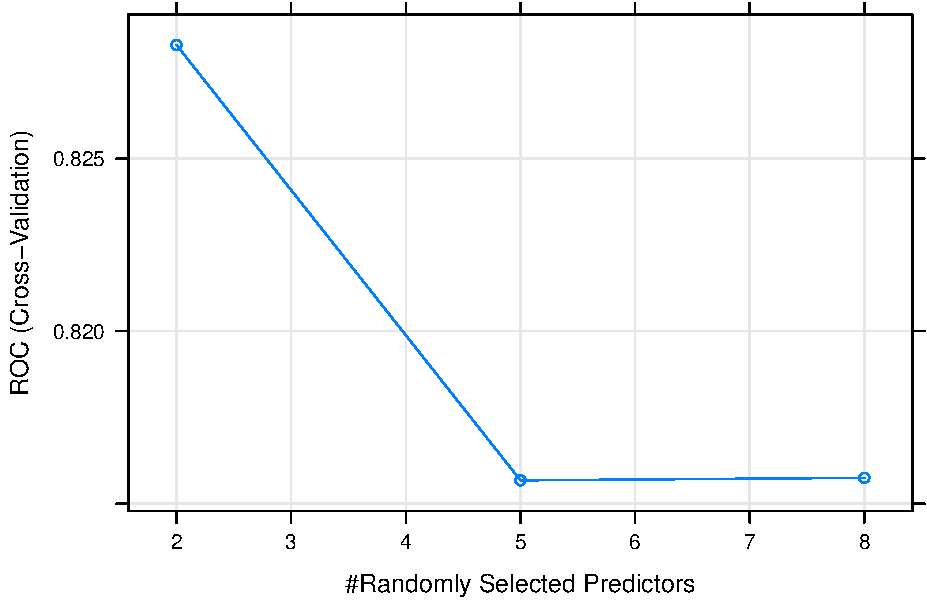
\includegraphics{SEMINAR_SERIES_files/figure-latex/plotrf-1.pdf}

\chapter{Feature Importance}\label{feature-importance}

Another advantage of using the caret \textbf{train} function is that it
provides a method to determine variable importance. This is useful when
considering what features to include or not when building a model. If we
summarize a given model, our myglm\_caret model, we'll see that some of
our predictors are not significant.

We could use the \textbf{varImp} to use statistics generated by the
specific modeling process itself. For more complex modeling techniques
this winds up being very useful since digging into the model diagnostics
can be daunting - although quite useful.

\begin{Shaded}
\begin{Highlighting}[]
\KeywordTok{varImp}\NormalTok{(myglm_caret)}
\end{Highlighting}
\end{Shaded}

\begin{verbatim}
## glm variable importance
## 
##          Overall
## glucose   100.00
## mass       61.38
## pregnant   41.70
## pedigree   36.00
## pressure   31.63
## age        17.81
## insulin    13.48
## triceps     0.00
\end{verbatim}

If you wanted to see how the different models rates the significance of
predictor variables then you can easily plot them.

\begin{Shaded}
\begin{Highlighting}[]
\KeywordTok{library}\NormalTok{(gridExtra)}
\NormalTok{p1 <-}\StringTok{ }\KeywordTok{plot}\NormalTok{(}\KeywordTok{varImp}\NormalTok{(myglm_caret),}\DataTypeTok{main=}\StringTok{"varImp for glm"}\NormalTok{)}
\NormalTok{p2 <-}\StringTok{ }\KeywordTok{plot}\NormalTok{(}\KeywordTok{varImp}\NormalTok{(myrf_caret),}\DataTypeTok{main=}\StringTok{"varImp for Rf"}\NormalTok{)}
\KeywordTok{grid.arrange}\NormalTok{(p1,p2,}\DataTypeTok{ncol=}\DecValTok{2}\NormalTok{)}
\end{Highlighting}
\end{Shaded}

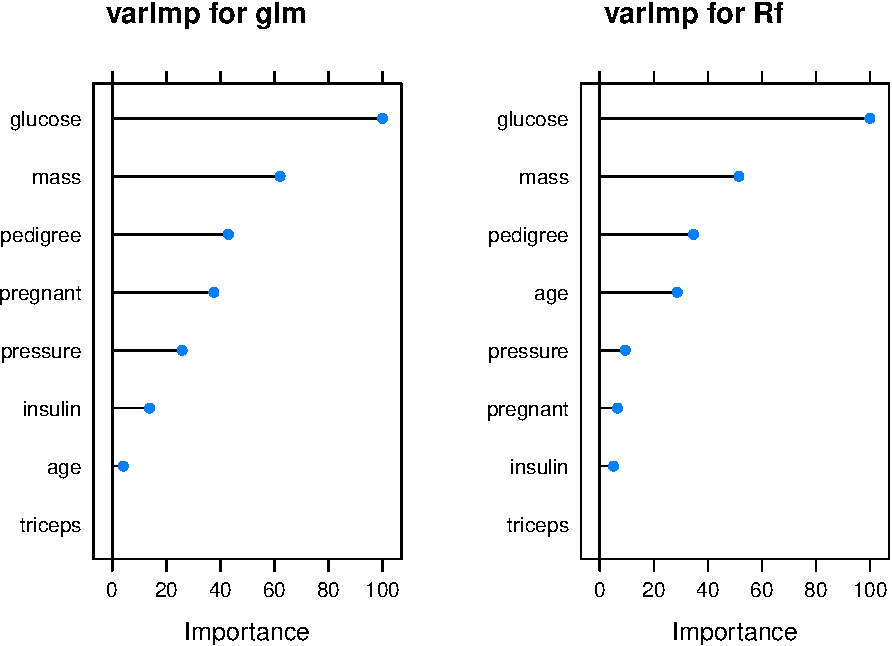
\includegraphics{SEMINAR_SERIES_files/figure-latex/plotfeat-1.pdf}

\subsection{Feature Elimination}\label{feature-elimination}

The caret package also supports ``recursive feature elimination'' which
automates the selection of optimal features. This can be controversial
since such a process could work at the expense of important statistical
considerations. However, it remains a tool in the Machine Learning
toolbox. Let's work though an example of this using caret functions.
First, we'll remove highly correlated predictor variables from
consideration.

\begin{Shaded}
\begin{Highlighting}[]
\NormalTok{correlationMatrix <-}\StringTok{ }\KeywordTok{cor}\NormalTok{(pm[,}\DecValTok{1}\OperatorTok{:}\DecValTok{8}\NormalTok{])}

\CommentTok{# summarize the correlation matrix}
\KeywordTok{print}\NormalTok{(correlationMatrix)}
\end{Highlighting}
\end{Shaded}

\begin{verbatim}
##             pregnant    glucose   pressure     triceps     insulin
## pregnant  1.00000000 0.12945867 0.14128198 -0.08167177 -0.07353461
## glucose   0.12945867 1.00000000 0.15258959  0.05732789  0.33135711
## pressure  0.14128198 0.15258959 1.00000000  0.20737054  0.08893338
## triceps  -0.08167177 0.05732789 0.20737054  1.00000000  0.43678257
## insulin  -0.07353461 0.33135711 0.08893338  0.43678257  1.00000000
## mass      0.01768309 0.22107107 0.28180529  0.39257320  0.19785906
## pedigree -0.03352267 0.13733730 0.04126495  0.18392757  0.18507093
## age       0.54434123 0.26351432 0.23952795 -0.11397026 -0.04216295
##                mass    pedigree         age
## pregnant 0.01768309 -0.03352267  0.54434123
## glucose  0.22107107  0.13733730  0.26351432
## pressure 0.28180529  0.04126495  0.23952795
## triceps  0.39257320  0.18392757 -0.11397026
## insulin  0.19785906  0.18507093 -0.04216295
## mass     1.00000000  0.14064695  0.03624187
## pedigree 0.14064695  1.00000000  0.03356131
## age      0.03624187  0.03356131  1.00000000
\end{verbatim}

\begin{Shaded}
\begin{Highlighting}[]
\CommentTok{# find attributes that are highly corrected }
\CommentTok{# (ideally >0.75)}
\NormalTok{highlyCorrelated <-}\StringTok{ }\KeywordTok{findCorrelation}\NormalTok{(correlationMatrix,}
                                    \DataTypeTok{cutoff=}\FloatTok{0.5}\NormalTok{)}

\CommentTok{# print indexes of highly correlated attributes}
\KeywordTok{print}\NormalTok{(highlyCorrelated)}
\end{Highlighting}
\end{Shaded}

\begin{verbatim}
## [1] 8
\end{verbatim}

\subsection{The rfe Function}\label{the-rfe-function}

Let's apply the RFE method on the Pima Indians Diabetes data set. The
algorithm is configured to explore all possible subsets of the
attributes. All 8 attributes are selected in this example, although in
the plot showing the accuracy of the different attribute subset sizes,
we can see that just 4 attributes gives almost comparable results

\begin{Shaded}
\begin{Highlighting}[]
\NormalTok{rfFuncs}\OperatorTok{$}\NormalTok{summary <-}\StringTok{ }\NormalTok{twoClassSummary}
\NormalTok{control <-}\StringTok{ }\KeywordTok{rfeControl}\NormalTok{(}\DataTypeTok{functions=}\NormalTok{rfFuncs, }
                      \DataTypeTok{method=}\StringTok{"cv"}\NormalTok{, }
                      \DataTypeTok{number=}\DecValTok{4}\NormalTok{)}

\CommentTok{# run the RFE algorithm}
\NormalTok{results <-}\StringTok{ }\KeywordTok{rfe}\NormalTok{(pm[,}\DecValTok{1}\OperatorTok{:}\DecValTok{8}\NormalTok{], }
\NormalTok{               pm[,}\DecValTok{9}\NormalTok{], }
               \DataTypeTok{sizes=}\KeywordTok{c}\NormalTok{(}\DecValTok{1}\OperatorTok{:}\DecValTok{8}\NormalTok{), }
               \DataTypeTok{rfeControl=}\NormalTok{control,}
               \DataTypeTok{metric=}\StringTok{"ROC"}\NormalTok{)}

\CommentTok{# summarize the results}
\KeywordTok{print}\NormalTok{(results)}
\end{Highlighting}
\end{Shaded}

\begin{verbatim}
## 
## Recursive feature selection
## 
## Outer resampling method: Cross-Validated (4 fold) 
## 
## Resampling performance over subset size:
## 
##  Variables    ROC  Sens   Spec   ROCSD  SensSD  SpecSD Selected
##          1 0.7103 0.854 0.4328 0.03105 0.02477 0.08175         
##          2 0.7598 0.820 0.5410 0.02825 0.04357 0.02239         
##          3 0.8022 0.840 0.5634 0.02402 0.05102 0.05764         
##          4 0.8085 0.832 0.6082 0.02167 0.04131 0.06934         
##          5 0.8159 0.842 0.5858 0.02794 0.03290 0.08118         
##          6 0.8202 0.846 0.5858 0.02464 0.02723 0.06017         
##          7 0.8259 0.858 0.5896 0.02386 0.03993 0.08914         
##          8 0.8284 0.858 0.5821 0.02484 0.02800 0.08872        *
## 
## The top 5 variables (out of 8):
##    glucose, mass, age, pregnant, pedigree
\end{verbatim}

\begin{Shaded}
\begin{Highlighting}[]
\CommentTok{# list the chosen features}
\KeywordTok{predictors}\NormalTok{(results)}
\end{Highlighting}
\end{Shaded}

\begin{verbatim}
## [1] "glucose"  "mass"     "age"      "pregnant" "pedigree" "insulin" 
## [7] "triceps"  "pressure"
\end{verbatim}

\begin{Shaded}
\begin{Highlighting}[]
\CommentTok{# plot the results}
\KeywordTok{plot}\NormalTok{(results, }\DataTypeTok{type=}\KeywordTok{c}\NormalTok{(}\StringTok{"g"}\NormalTok{, }\StringTok{"o"}\NormalTok{))}
\end{Highlighting}
\end{Shaded}

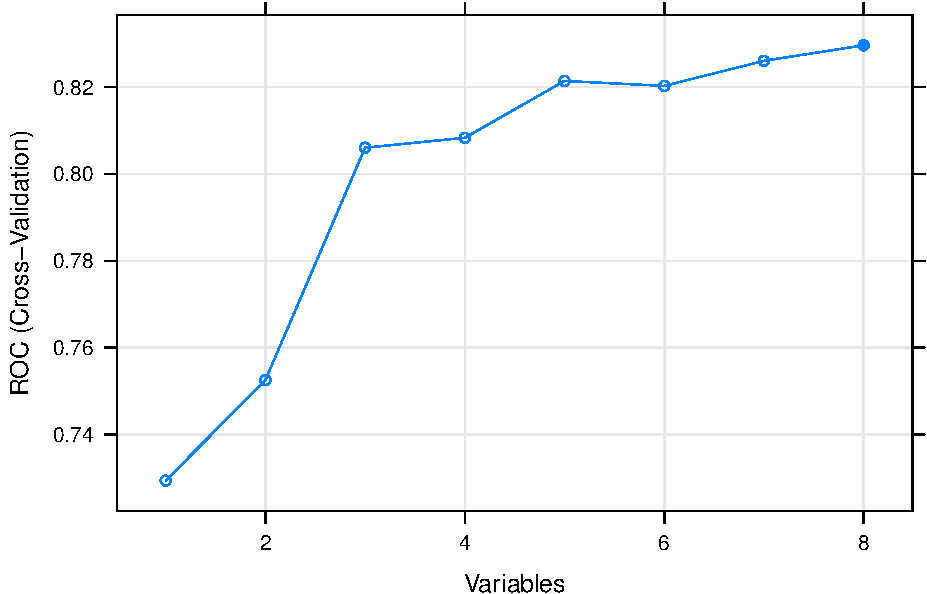
\includegraphics{SEMINAR_SERIES_files/figure-latex/rfe1-1.pdf}

\chapter{Comparing Models}\label{comparing-models}

One of the more frequent activities in Machine Learning relates to
setting up ``shoot ours'' between different models to see which one will
perform the best. This is something we could do without \textbf{caret}
but the package does help accomplish this using a standard interface.
We'll keep using the Pima Indians Data and (re)build a few models. We'll
use a common \textbf{control} object as well as a seed to maintain
reproducibility.

\begin{Shaded}
\begin{Highlighting}[]
\NormalTok{control <-}\StringTok{ }\KeywordTok{trainControl}\NormalTok{(}\DataTypeTok{method=}\StringTok{"cv"}\NormalTok{, }
                        \DataTypeTok{number=}\DecValTok{5}\NormalTok{, }
                        \DataTypeTok{summaryFunction =}\NormalTok{ twoClassSummary,}
                        \DataTypeTok{classProbs =} \OtherTok{TRUE}\NormalTok{)}

\CommentTok{# Train the glm model}
\KeywordTok{set.seed}\NormalTok{(}\DecValTok{7}\NormalTok{)}
\NormalTok{model_glm <-}\StringTok{ }\KeywordTok{train}\NormalTok{(diabetes }\OperatorTok{~}\StringTok{ }\NormalTok{., }
                   \DataTypeTok{data=}\NormalTok{pm, }
                   \DataTypeTok{method=}\StringTok{"glm"}\NormalTok{, }
                   \DataTypeTok{metric=}\StringTok{"ROC"}\NormalTok{,}
                   \DataTypeTok{trControl=}\NormalTok{control)}

\CommentTok{# Train the Decision Tree <odel}
\KeywordTok{set.seed}\NormalTok{(}\DecValTok{7}\NormalTok{)}
\NormalTok{model_rpart <-}\StringTok{ }\KeywordTok{train}\NormalTok{(diabetes}\OperatorTok{~}\NormalTok{., }
                  \DataTypeTok{data=}\NormalTok{pm, }
                  \DataTypeTok{method=}\StringTok{"rpart"}\NormalTok{, }
                  \DataTypeTok{metric=}\StringTok{"ROC"}\NormalTok{,}
                  \DataTypeTok{trControl=}\NormalTok{control)}

\CommentTok{# Train the Random Forest model}
\KeywordTok{set.seed}\NormalTok{(}\DecValTok{7}\NormalTok{)}
\NormalTok{model_rf <-}\StringTok{ }\KeywordTok{train}\NormalTok{(diabetes}\OperatorTok{~}\NormalTok{., }
                  \DataTypeTok{data=}\NormalTok{pm, }
                  \DataTypeTok{method=}\StringTok{"rf"}\NormalTok{, }
                  \DataTypeTok{metric=}\StringTok{"ROC"}\NormalTok{,}
                  \DataTypeTok{trControl=}\NormalTok{control)}

\CommentTok{# Use the resamples function to prep for comparisons}
\NormalTok{results <-}\StringTok{ }\KeywordTok{resamples}\NormalTok{(}\KeywordTok{list}\NormalTok{(}\DataTypeTok{GLM   =}\NormalTok{ model_glm, }
                          \DataTypeTok{RPART =}\NormalTok{ model_rpart, }
                          \DataTypeTok{RF    =}\NormalTok{ model_rf))}
\end{Highlighting}
\end{Shaded}

Now we can easily look at how well the different models compare:

\begin{Shaded}
\begin{Highlighting}[]
\CommentTok{# summarize the distributions}
\KeywordTok{summary}\NormalTok{(results)}
\end{Highlighting}
\end{Shaded}

\begin{verbatim}
## 
## Call:
## summary.resamples(object = results)
## 
## Models: GLM, RPART, RF 
## Number of resamples: 5 
## 
## ROC 
##            Min.   1st Qu.    Median      Mean   3rd Qu.      Max. NA's
## GLM   0.8007407 0.8042593 0.8392593 0.8344745 0.8479245 0.8801887    0
## RPART 0.6974074 0.7090566 0.7329245 0.7411184 0.7579630 0.8082407    0
## RF    0.7878704 0.8193519 0.8359434 0.8323997 0.8368519 0.8819811    0
## 
## Sens 
##       Min. 1st Qu. Median  Mean 3rd Qu. Max. NA's
## GLM   0.85    0.87   0.89 0.886    0.89 0.93    0
## RPART 0.75    0.82   0.85 0.836    0.88 0.88    0
## RF    0.81    0.84   0.87 0.856    0.88 0.88    0
## 
## Spec 
##            Min.   1st Qu.    Median      Mean   3rd Qu.      Max. NA's
## GLM   0.5555556 0.5555556 0.5740741 0.5747729 0.5849057 0.6037736    0
## RPART 0.4444444 0.5471698 0.5660377 0.5596785 0.5740741 0.6666667    0
## RF    0.5000000 0.5740741 0.5925926 0.6012579 0.6415094 0.6981132    0
\end{verbatim}

\begin{Shaded}
\begin{Highlighting}[]
\CommentTok{# boxplots of results}
\KeywordTok{bwplot}\NormalTok{(results)}
\end{Highlighting}
\end{Shaded}

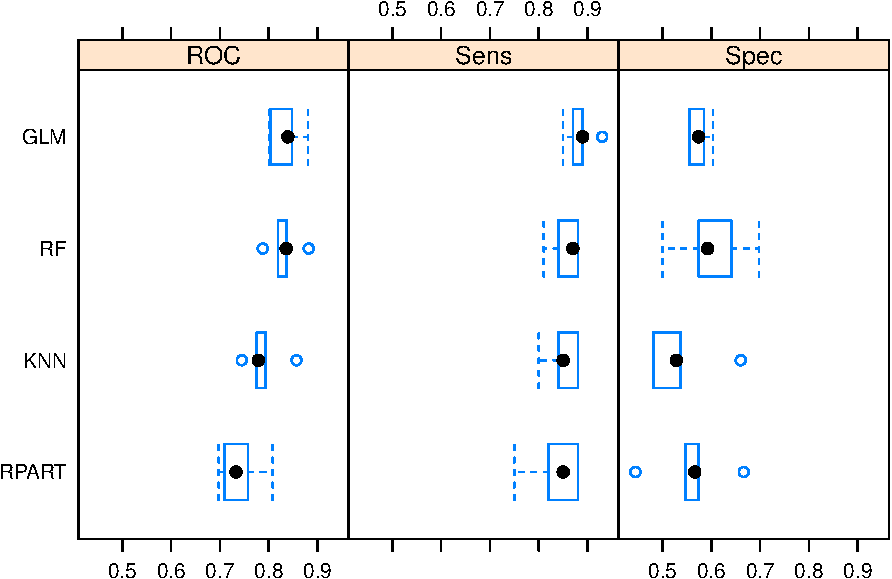
\includegraphics{SEMINAR_SERIES_files/figure-latex/summcomp-1.pdf}

\begin{Shaded}
\begin{Highlighting}[]
\CommentTok{# dot plots of results}
\KeywordTok{dotplot}\NormalTok{(results)}
\end{Highlighting}
\end{Shaded}

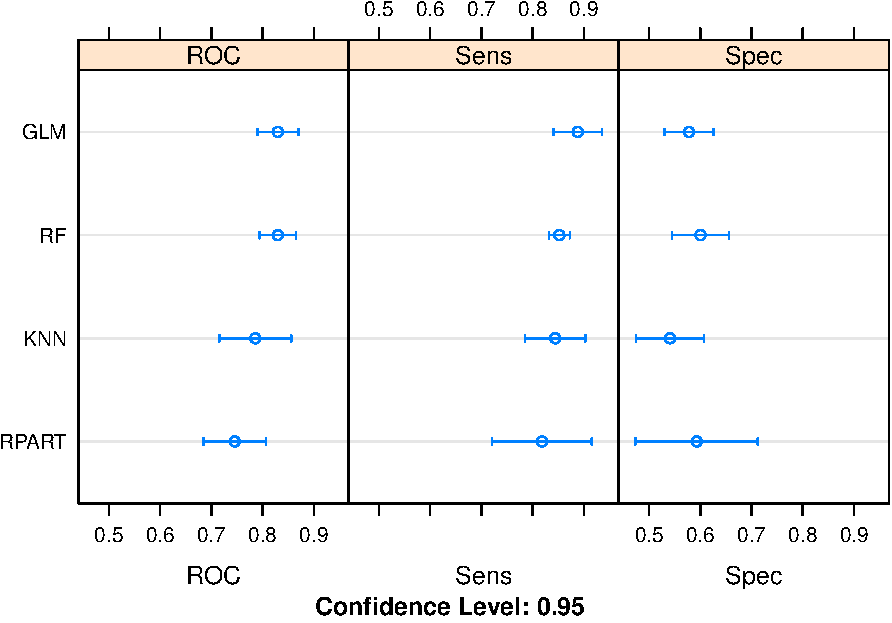
\includegraphics{SEMINAR_SERIES_files/figure-latex/summcomp-2.pdf}

\bibliography{book.bib,packages.bib}


\end{document}
